% !TEX TS-program = xelatex
% !TEX encoding = UTF-8 Unicode
% !Mode:: "TeX:UTF-8"
\documentclass[bachelor,nocolorlinks, printoneside]{seuthesis} % 本科

% \documentclass[master]{seuthesis} % 硕士
% \documentclass[doctor]{seuthesis} % 博士
% \documentclass[engineering]{seuthesis} % 工程硕士
\usepackage{CJK,CJKnumb}
\usepackage{amsmath}
% \usepackage[table,xcdraw]{xcolor}
\usepackage{amsfonts} 
\usepackage{bm} 
\usepackage{algorithm}
\usepackage{algorithmicx}
\usepackage{algpseudocode}
\usepackage{subcaption}
\usepackage{bigstrut}
\usepackage{tabularx}
\usepackage{bookmark}


\floatname{algorithm}{算法}
\renewcommand{\algorithmicrequire}{\textbf{输入:}}
\renewcommand{\algorithmicensure}{\textbf{输出:}}
 % 这里是导言区

\begin{document}

%# -*- coding: utf-8-unix -*-
\categorynumber{000} % 分类采用《中国图书资料分类法》
\UDC{000}            %《国际十进分类法UDC》的类号
\secretlevel{公开}    %学位论文密级分为"公开"、"内部"、"秘密"和"机密"四种
\studentid{09015131}   %学号要完整,前面的零不能省略。

\title{集群缓存系统负载均衡算法的设计与实现}{}{CW-Cache: Column-wise Load Balancing for Structured Data}{}
\author{郑云川}{Yunchuan Zheng}
\advisor{肖卿俊}{副教授}{Qingjun Xiao}{Associate Prof.}
\coadvisor{王威}{助理教授}{Wei Wang}{Assistant Prof.}

% \degree{工学硕士} % 详细学位名称
\major[12em]{计算机科学与技术}
\defenddate{答辩日期}
\authorizedate{学位授予日期}
\department{计算机科学与工程}{Computer Science and Engineering}
\duration{2019年1月—2019年6月}
\address{HKUST}
% \thanks{本论文获国家XXX计划项目(2012AA00A00)和国家杰出青年科学基金项目(01234567)资助。}

\maketitle

%# -*- coding: utf-8-unix -*-
%%==================================================
%% abstract.tex for seuthesis Bachelor Thesis
%%==================================================

\begin{abstract}{集群缓存,列级别,负载均衡,结构化数据}

    目前越来越多的数据密集型集群部署内存计算方案来提高I/O性能,在集群内存使用缓存是一种普遍做法。然而负载不均这一集群缓存中常见的问题则会损害缓存带来的好处。学术界应对这一问题的方法包括将热门的文件复制多份、用存储编码为文件创建同等分区、选择性地将文件分割成多份来分散存储。然而这些方法均关注一般意义上的文件的负载均衡,而本文关注的是结构化数据的负载均衡,根据数据表中各个列的访问热度倾斜实现列级别的负载均衡。我们的解决方案称为CW-Cache,将数据表中访问热度排在前$K$的列一起复制$r$份缓存在集群中。我们通过数学建模,在数据表各个列的热度确定的情况下,高效地计算出最优的$K$和$r$——二者太小不足以实现负载均衡,太大则会增大内存开销。我们在分布式内存文件系统Alluxio上实现了CW-Cache,评估表明相比原生Alluxio,我们的CW-Cache系统能够降低SQL任务执行时间达平均12\%,负载不均衡程度优化26\%。
    \end{abstract}
    
    \begin{englishabstract}{Cluster Cache, Column-wise, Load Balancing,  Structured Data}
    
    Nowadays, more and more data-intensive clusters employ in-memory solutions to improve I/O performance and a common approach is using cache in cluster memories. Nevertheless, routinely observed load imbalance will degrade the benefits of caching. Solutions that the academic deal with this problem include copying multiple replicas of hot files, creating parity chunks using storage codes and selectively partitioning files and caching them across  the clusters. Yet, they focus on load balance of general files, while this paper cares about load balance of structured data. We aimed to achieve column-wise load balance based on the skewed popularities of columns. Our solution, called CW-Cache, bundle columns with their popularities in the top $K$ list with a replicative factor of $r$. Through modeling, we effectively calculate the optimal $K$ and $r$ given popularities of each column -- too small leads to load imbalance, while too large results in high memory costs. We implemented CW-Cache atop Alluxio, a popular in-memory distributed storage for data-intensive clusters. Our evaluation shows that, compared with Alluxio, CW-Cache could reduce SQL query execution time by 12\% in average and improve load balancing by around 26\%.
    \end{englishabstract}


\tableofcontents

% \begin{terminology}
% \begin{table}[h]
% \renewcommand\arraystretch{1.5}
% %\Large
% \begin{tabular}{>{\LARGE}m{0.2\textwidth} <{\centering}m{0.7\textwidth}}
% a & 如同汉字起源于象形,拉丁字母表中的每个字母一开始都是描摹某种动物或物体形状的图画\\

% b&和A一样,字母B也可以追溯到古代腓尼基。在腓尼基字母表中B叫beth,代表房屋,在希伯来语中B也叫beth,也含房屋之意。\\

% c& 字母C在腓尼基人的文字中叫gimel,代表骆驼。它在字母表中的排列顺序和希腊字母Γ(gamma)相同,实际上其字形是从后者演变而来的。C在罗马数字中表示100。\\

% d&D在古时是描摹拱门或门的形状而成的象形符号,在古代腓尼基语和希伯来语中叫做daleth,是“门”的意思,相当于希腊字母Δ(delta)。\\

% \end{tabular}
% %\caption{my table}
% \end{table}
% \end{terminology}


\begin{Main} % 开始正文

%# -*- coding: utf-8-unix -*-
%%==================================================
%% introduction.tex for seuthesis Bachelor Thesis
%%==================================================

\chapter{前言}
\label{chp:intro}

本章是课题的前言部分。在此章中,首先介绍了课题的实际背景,接下来是课题的目的和意义,并且对当前的研究现状做了简要调研与分析,最后介绍了课题的主要研究内容。

\section{课题背景}

\subsection{大数据}

\par 因为技术的不断发展,包括物联网,云计算的崛起\cite{botta2016integration}、智能设备的流行等,在当今时代各种各样不同的领域(例如健康领域、政府、社交网络、营销、财务),每一天都在以前所未有的速度产生大量的数据\cite{oussous2018big}。从海量的数据中,我们能够挖掘出大量有用的规律,对人们的生活产生积极的影响。在大数据革命之前,大公司很难将他们的数据存档保存较长时间,也难以管理庞大的数据集。传统技术存储能力有限,管理工具很昂贵,它们缺乏大数据背景所需要的灵活性、可扩展性和性能。事实上,大数据管理需要大量资源,新方法和强大技术,进一步来说,大数据需要清洗,处理,分析,保护数据,并提供对大量不断发展的数据集的细粒度访问\cite{oussous2018big}。为了应对大数据带来的机遇和挑战,学界和业界开展了大量的研究与开发工作,发展出来众多技术,提供了很多成熟的模型、框架、软件。典型的互联网大数据平台(如图~\ref{fig:frame})从上至下大致可分为三个部分:

\begin{itemize}
	\item 数据采集:将应用程序产生的数据和日志等同步到大数据系统,同步时数据可能还需经过清洗、转化等过程;
	\item 数据处理:包括大数据存储、离线计算和流式计算等;
	\item 数据输出与展示:大数据经过处理后将有价值的信息存入数据库,通过数据库给用户提供所需信息,或者给运营、决策人员提供所需信息。
\end{itemize}

\par 此外,将三个部分整合起来的是大数据任务调度管理系统,它会管理数据的同步、集群资源的分配等等。
\begin{figure}[ht]
	\centering
	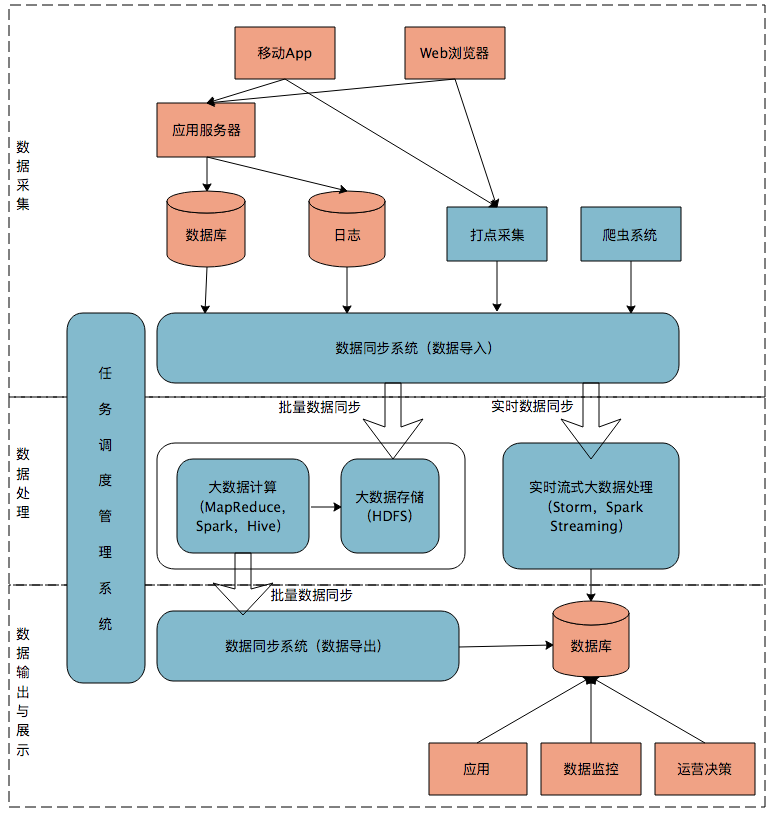
\includegraphics[width=0.50\paperwidth]{img/introduction/big-data-framework.png}
	\caption{典型的互联网大数据平台架构。}
	\label{fig:frame}
	%\vspace{-.15in}
\end{figure}

% \subsection{内存缓存}
% \par 在大数据平台中(图~\ref{fig:frame}),数据处理是非常重要的一环,实现对数据的高效清洗、存储和挖掘是这个环节的目标。对计算能力的需求随着数据量的急剧增加而增加,但是单机的处理能力和 I/O 性能并没有跟上这种增长,越来越多的企业不得不向外扩展他们的计算至集群模式\cite{Zaharia:2016:AFG:3002856}。集群环境对编程平台提出了更高的要求,主要有三方面,一是程序需要并行化执行,二是需要强大的容错能力,三是动态地扩展和缩减计算资源,为此,越来越多的编程模型被设计出来。在存储方面,谷歌提出了分布式文件系统GFS(Google File System)\cite{51},对应的开源实现是HDFS(Hadoop File System)\cite{hdfs},它实现了对成千上万台机器上的大规模数据进行高效地存储、访问,并且具有高度容错能力。计算框架方面,起初,谷歌的 MapReduce\cite{dean2008mapreduce}提出了一种简单通用而且能够自动处理故障的批处理计算模型,但是它将中间以及最终结果保存在磁盘上,消耗大量I/O时间,不利于重用计算结果。Spark\cite{Zaharia:2016:AFG:3002856}、Pregel\cite{malewicz2010pregel}等采用内存计算方案来加速计算,实现数据的重复利用。很多系统的性能瓶颈主要是I/O,包括磁盘读写和网络远程读写的延迟,为了进一步提高性能,一种典型的方法是部署缓存,并且将数据在分布式集群中服务器的内存进行缓存\cite{ananthanarayanan2012pacman},并且尽力实现计算任务和数据的本地性(locality)。内存的读写速度远高于磁盘,将计算与数据部署在相同的机器也能节约网络开销。
\par 在大数据平台中(图~\ref{fig:frame}),数据处理是非常重要的一环,实现对数据的高效清洗、存储和挖掘是这个环节的目标。对计算能力的需求随着数据量的急剧增加而增加,但是单机的处理能力和 I/O 性能并没有跟上这种增长,越来越多的企业不得不向外扩展他们的计算至集群模式\cite{Zaharia:2016:AFG:3002856}。集群环境对编程平台提出了更高的要求,主要有三方面,一是程序需要并行化执行,二是需要强大的容错能力,三是动态地扩展和缩减计算资源,为此,越来越多的编程模型被设计出来。在存储方面,谷歌提出了分布式文件系统GFS(Google File System)\cite{51},对应的开源实现是HDFS(Hadoop File System)\cite{hdfs},它实现了对成千上万台机器上的大规模数据进行高效地存储、访问,并且具有高度容错能力。计算框架方面,起初,谷歌的 MapReduce\cite{dean2008mapreduce}提出了一种简单通用而且能够自动处理故障的批处理计算模型,但是它将中间以及最终结果保存在磁盘上,消耗大量I/O时间,不利于重用计算结果。Spark\cite{Zaharia:2016:AFG:3002856}、Pregel\cite{malewicz2010pregel}等采用内存计算方案来加速计算,实现数据的重复利用。

\subsection{集群缓存}
\par 由于近来数据中心架构的改进~\cite{singh2015jupiter} 和高速网络设备的出现\cite{huawei_nuwa,asanovic2014firebox,alistarh15a},网络带宽和存储器I/O带宽之间的差距正在迅速减小~\cite{latency_trends,p802_3ba,Han13a,Gao16a},因此,云计算系统的性能瓶颈正迅速从网络转变为存储器I/O。先前的工作证明从本地硬盘读取数据相比网络远程读取并没有显著的优势 ~\cite{Ananthanarayanan11a},这个结论同样适用于固态硬盘(SSD)。最近的一个研究~\cite{Jonas17a} 表明将数据存储在EC2实例的一个本地SSD上甚至比把数据写到Amazon S3 ~\cite{amazons3}上还要慢,Amazon S3是一个远程的提供了PUT/GET接口的对象存储服务。当磁盘本地化变得无关紧要,云端对象存储如 Amazon S3~\cite{amazons3}、 Windows Azure Storage~\cite{azure_storage}、和OpenStack Swift~\cite{swift}等,逐渐取代与计算同地的存储(尤其是HDFS~\cite{shvachko2010hadoop}),作为数据密集型应用的首选存储方式。

\par 然而,云端对象存储在磁盘I/O上依然是瓶颈~\cite{rashmi2016ec},因为从磁盘读数据比从内存读数据慢至少两个数量级,考虑到这个问题,集群缓存系统,例如Alluxio~\cite{alluxio}、Memcached~\cite{memcached}和Redis~\cite{redis},被越来越多的云端对象存储系统部署来提供内存速度级别的低延迟数据访问,而集群缓存系统面对的一个很大的挑战便是如何实现负载均衡。

\par 一个能够实现分布式内存缓存的系统是Alluxio。Alluxio\cite{li2014tachyon}是开源的分布式内存文件系统,旨在作为上层繁多的计算框架(如MapReduce、Apache Spark、Apache Storm、Apche Mahout等)与底层存储层(如文件系统、对象存储、键值对存储等)的中间层,提供统一的文件读写的接口,实现全局的数据访问、高效的内存数据共享、跨应用的数据管理、高效的网络带宽利用,它借助“血缘关系”、检查点机制提供强大的容错能力。鉴于这些特点,alluxio也非常适合作为内存缓存系统,进一步加速数据分析应用。


\subsection{负载均衡}
\par 上一小节提及的Apache Spark等内存计算方案的一个重要挑战是负载不均,在先前工作 
\cite{ananthanarayanan2011scarlett,rashmi2016ec} 中,研究人员已经发现了生产集群中负载不均的两个来源:\emph{文件热门程度差别} 和 \emph{网络流量不均}。

\par 在数据中心中,我们普遍观察到,文件(数据对象)热门程度差别极大,并且遵循Zipf分布~\cite{rashmi2016ec, ananthanarayanan2011scarlett, ananthanarayanan2012pacman, li2014tachyon},也就是说,数据访问的大部分请求是由一小部分非常热门的文件贡献的。图~\ref{fig:Yahoo_trace}描述了Yahoo!集群查询数据集~\cite{yahoo!_trace}中文件的热门程度和文件大小的分布,从这个数据集可以得到某两个月内对超过四千万个文件的访问的统计数据。我们发现绝大多数文件($\sim 78\%$)存储的是冷门数据,很少被访问($<10$ times),只有 $2\%$ 的文件有高访问量($\ge100$),这些文件通常比那些冷门的文件大很多($15$-$30 \times$)。由于这些文件较大的体积和较高的访问量,缓存这些文件的服务器很容易负荷过重。

\begin{figure}[t]
\centering
   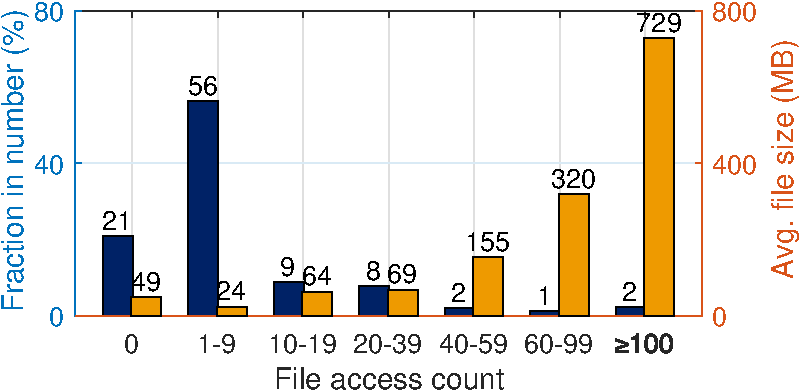
\includegraphics[width=0.5\textwidth]{img/introduction/Yahoo_pop-eps-converted-to.pdf}
   \caption{Yahoo!集群上观察到的文件热门程度(蓝色)和文件大小(橙色)的分布~\cite{yahoo!_trace}.}
\label{fig:Yahoo_trace}
\vspace{-.1in}
\end{figure}

\par 这个问题由于网络负载不均而加重,这在生产环境的数据中心非常普遍~\cite{Kandula09a,Chowdhury13a,Greenberg09a,rashmi2016ec},例如,在研究~\cite{rashmi2016ec}中,研究者测量了Facebook一个集群所有上行和下行链路中最大利用率和平均利用率的比值,结果表明这个比值在半数以上的时间里保持在4.5以上,这意味着严重的负载不均。在SP-Cache~\cite{Yu:2018:SLR:3291656.3291658}的研究中,研究人员分别测量了在有无内存缓存的情况下,不同请求速率下的文件的平均读延迟,结果表明~\ref{fig:impact_of_imbalance}当集群负载不重时(每秒$5$个请求),内存缓存带来了显著性好处,降低平均读延迟达 $5\times$,然而,当负载骤然增大,集群中的热点机器变得突出,缓存带来的好处迅速减少,尤其当请求速率大于$9$,读延迟就由热点服务器的网络拥塞决定,内存缓存就变得\emph{无关紧要}。

\begin{figure}[t]
    \centering
    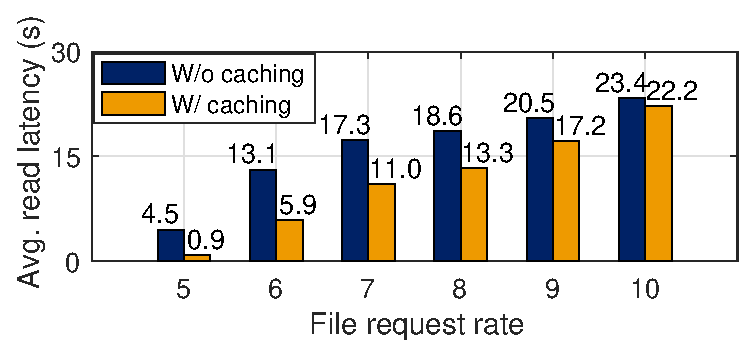
\includegraphics[width=0.8\textwidth]{img/introduction/latencies_under_imbalance}
    \caption{有/无缓存的情况下平均读延迟随着负载增加而增加。}
    \label{fig:impact_of_imbalance}
    \vspace{-.15in}
\end{figure}

\section{研究现状}

\par 当今的数据并行集群依赖内存计算方案来进行高性能的数据分析工作\cite{li2014tachyon, presto, Zaharia:2016:AFG:3002856, power2010piccolo, memcached, memsql},通过将数据对象缓存在内存中, I/O 密集型应用相对于传统的磁盘解决方案能够获得数量级的性能提升\cite{li2014tachyon, Zaharia:2016:AFG:3002856, power2010piccolo}

\par 然而,内存计算方案面对的一个严峻的挑战是缓存服务器之间严重的负载不均衡。在生产集群中,数据对象有严重的热门程度差别,这意味着对一小部分非常热门的文件访问占据了总访问的很大一部分\cite{rashmi2016ec, ananthanarayanan2011scarlett, ananthanarayanan2012pacman}。存储有热门文件的缓存服务器因此变为访问热点,这个问题因为网络的负载不均衡而进一步恶化。据报道,在 Facebook 的一个集群中,负载最重的链路的利用率在 $50\%$ 的时间里比 平均链路利用率高出 4.5 倍\cite{rashmi2016ec}。访问热点和网络负载不均导致了 I/O 性能极大下降,这甚至可能会抵消内存计算带来的性能提升。

\par 因此,保证负载均衡是提高集群缓存性能的关键,这方面的解决方案包括选择性复制\cite{ananthanarayanan2011scarlett}、纠删码\cite{rashmi2016ec}和选择分割\cite{Yu:2018:SLR:3291656.3291658},前二者是借助缓存冗余来减缓访问热点机器的负担,第三个是根据文件的热门程度将文件分割成不同份数,并随机放置在不同服务器上,分散请求负载。

\subsection{选择复制}

\par 选择复制方案基于文件的热门程度对文件进行复制~\cite{ananthanarayanan2011scarlett,hong2013understanding},也就是说,一个文件的访问频率越高,它会越多被复制,并分散在集群中,一个文件的读请求就能随机选择一台含有这个文件副本的服务器提供服务。这样,读请求的负载就被均匀分散,提高负载均衡。

\par 虽然选择复制已被证明对于基于磁盘的存储系统是有效的~\cite{ananthanarayanan2011scarlett},但是因为复制带来了高额的内存开销,它在集群缓存上表现不佳~\cite{huang2014characterizing,rashmi2016ec}。研究~\cite{Yu:2018:SLR:3291656.3291658}的实验得出,内存开销的 \emph{线性增加}(热门文件副本数增加)换来了读延迟的 \emph{亚线性降低},而且热门文件的体积通常比较大(图~\ref{fig:Yahoo_trace})。

\subsection{纠删码}

\par 有研究利用\emph{纠删码}~\cite{huang2012erasure,sathiamoorthy2013xoring} 来实现缓存服务器之间的负载均衡且避免产生高额的内存开销。一个$(k,n)$的纠删码方案能够将一个文件均匀地切分成$k$份,然后计算同样大小的$n-k$个 \emph{奇偶校验分区},原始文件能通过解码$n$份中的任意$k$份来获得,从而使得读请求的负载被分散到$n$台服务器上。内存的额外开销是$(n-k)/k$,在实际设定中比选择复制低(至少 $1\times$)。
\par 这个方法的一个有效实现是EC-Cache~\cite{rashmi2016ec},它在读取文件时通过\emph{迟绑定}来减轻落后机器的影响,换句话说,EC-Cache随机读取文件分区中的$k+1$份,等待其中的$k$份完成读取,而不是恰好读取$k$份。EC-Cache在读文件的中位和尾延迟都比选择复制低很多~\cite{rashmi2016ec}。然而,EC-Cache在读(写)时带来巨大的解码(编码)的额外开销,即使有高度优化的编码和实现方案,解码的开销仍会对读请求产生高达$30\%$~\cite{rashmi2016ec}延迟。

\subsection{选择分割}

\par 研究~\cite{Yu:2018:SLR:3291656.3291658}中提出了SP-Cache来实现集群缓存的负载均衡,同时避免高额的内存和计算开销。它选择性地将热门文件根据其大小和热门程度,分割成一定数目的文件分区,随机缓存到不同的缓存服务器上,这样分散了读请求的负载,同时读操作可以并行,提升性能。SP-Cache建立了一个上限分析来量化平均延迟~\cite{Yu:2018:SLR:3291656.3291658},并基于这个推导设计了一个高效的算法来决定每个文件的最佳分区数量,文件分割的数目太小则不足以缓解热点机器的压力,分割的数目太大则容易受到慢机器的影响。此外它采集一段时间内集群中文件的访问数据,周期性地调整各个文件的分区数目。选择分割在不产生高额内存和计算开销的情况下实现可负载均衡,但因为其分割的特性,缓存无冗余,容错性依赖底层文件系统,且读取文件必须读取所有分区,会受到慢机器的影响。

\subsection{更细粒度负载均衡}

\par 以上方案都是针对一般意义上的文件来考虑负载均衡的,优点是非常通用,毋需考虑文件的语义,对于任何格式的文件都可以使用。它们负载均衡的粒度是文件,那么问题来了,能否在更细的粒度进行负载均衡,提高缓存效率呢?对于语义清晰的结构化数据,比如Parquet文件~\cite{parquet},如果在文件的内部列与列存在热门程度差异,列之间被共同查询的概率也存在差异,那么就没有必要去分割或者复制整个文件,只要对一个文件热门的这一部分,例如其中一列或者多列进行复制或者分割就行。这样能够节约内存,提高使用效率,因为内存总是有限的,而且一部分内存需要给计算任务使用,那么留作缓存的就更少了。这个目标的挑战在于底层分布式文件系统需要了解文件的语义,与上层的应用通信来获得这部分信息,可能产生一定程度的耦合,同时我们需要明智地决定对文件的哪些列进行复制或分割,在哪些机器上进行缓存。

\section{研究的目的与内容}
当前的大数据系统主要采用复制的方式来进行容错和负载均衡,而服务器内存的容量往往有限,缓存会产生不可忽视的内存开销。根据本项目的前期调研,生产集群中结构化数据(数据表)的不同列之间,热门程度(被访问热度)存在差异,列与列之间共同被查询的概率也存在差异,我们希望复制数据表中比较热门的列,而不是全表,并基于列与列之间被共同查询的概率设计一定的放置策略,实现以更少的内存,来获得相似的负载均衡效果的目标,从而节约资源,提高缓存效率。

总的来说,本课题的主要研究内容是上文提出的针对结构化数据文件的更细粒度(列级别)的负载均衡方案,具体来说:

\begin{itemize}
	\item 利用具有代表性的基准查询数据集,如TPC-DS, TPC-H等,测量数据表中列之间的查询频率,以及列与列之间被共同查询的频率,分析其中的统计及其他客观规律,为本项目的可行性奠定理论基础。
	\item 通过实验探究SQL查询过程中,数据的shuffle过程对任务执行时间的影响,证明数据表中相关列“捆绑放置”(bundle)的有效性,进一步强化项目的理论基础。
	\item 搭建Spark SQL~\cite{armbrust2015spark},Alluxio~\cite{alluxio},HDFS~\cite{shvachko2010hadoop}为主的集群系统,探索各组件之间通信协作机制,为项目方案实现奠定基础。
	\item 基于已有条件,主要在Alluxio~\cite{alluxio}基础上添加模块,使得Alluxio能够获取热门度以及关联性等信息,查阅相关文献,设计实现细粒度的负载均衡算法,并在AWS EC2搭建实验环境,进行测试。
\end{itemize}

\section{论文结构}

% \section{数学公式}
% \subsection{简单的数学公式}
% \textbf{卷积}(\textbf{convolution})在图像分析的线性方法中是一种重要的运算。卷积是一个积分,反映一个函数$f(t)$在另一个函数上$h(t)$移动时所重叠的量。函数$f$和$h$在有限域$[0,t]$上的$1D$卷积$f*h$由下式给出:
%  $$(f*h)(t) \equiv \int_0^t {f(\tau )h(t - \tau )d\tau } $$

% \subsection{带自动编号的公式}
% 这里可以限定在$[0,t]$区间,原因是我们假设负坐标部分的值是0。为了准确起见,我们还可以将卷积积分的上限扩展为$( - \infty ,\infty )$:
% \begin{equation}(f*h)(t) \equiv \int_{ - \infty }^\infty  {f(\tau )h(t - \tau )d\tau }  = \int_{ - \infty }^\infty  {f(t - \tau )h(\tau )d\tau }
%   \end{equation} 

% \subsection{带等号对齐的公式}
% 卷积可以推广到更高维。令$2D$函数$f$和$h$的卷积$g$记为$f*h$,则有:
% \begin{equation}
% \begin{aligned}
% (f*h)(x,y) &= \int_{ - \infty }^\infty  {\int_{ - \infty }^\infty  {f(a,b)h(x - a,y - b)} } dadb\\
%  &= \int_{ - \infty }^\infty  {\int_{ - \infty }^\infty  {f(x - a,y - b)h(a,b)} } dadb\\
% \end{aligned}
% \end{equation}

% \section{伪代码}
% 在写论文的时候我们通常要写伪代码,伪代码里面有时甚至还要包含数学公式(如根号一类的)。伪代码会自动找一个比较好的位置插入图片。

% \begin{algorithm}
%     \caption{用归并排序求逆序数}
%     \begin{algorithmic}[1] %每行显示行号
%         \Require $Array$数组,$n$数组大小
%         \Ensure 逆序数
%         \Function {MergerSort}{$Array, left, right$}
%             \State $result \gets 0$
%             \If {$left < right$}
%                 \State $middle \gets (left + right) / 2$
%                 \State $result \gets result +$ \Call{MergerSort}{$Array, left, middle$}
%                 \State $result \gets result +$ \Call{MergerSort}{$Array, middle, right$}
%                 \State $result \gets result +$ \Call{Merger}{$Array,left,middle,right$}
%             \EndIf
%             \State \Return{$result$}
%         \EndFunction
%         \State
%         \Function{Merger}{$Array, left, middle, right$}
%             \State $i\gets left$
%             \State $j\gets middle$
%             \State $k\gets 0$
%             \State $result \gets 0$
%             \While{$i<middle$ \textbf{and} $j<right$}
%                 \If{$Array[i]<Array[j]$}
%                     \State $B[k++]\gets Array[i++]$
%                 \Else
%                     \State $B[k++] \gets Array[j++]$
%                     \State $result \gets result + (middle - i)$
%                 \EndIf
%             \EndWhile
%             \While{$i<middle$}
%                 \State $B[k++] \gets Array[i++]$
%             \EndWhile
%             \While{$j<right$}
%                 \State $B[k++] \gets Array[j++]$
%             \EndWhile
%             \For{$i = 0 \to k-1$}
%                 \State $Array[left + i] \gets B[i]$
%             \EndFor
%             \State \Return{$result$}
%         \EndFunction
%     \end{algorithmic}
% \end{algorithm}

% \section{插入图片}
% 在使用该命令的时候,图片会自动找一个他觉得比较好的位置插入图片,我们就不需要担心前面改了文字之后后面的格式乱掉。
% \begin{figure}[htbp!]
% \centering 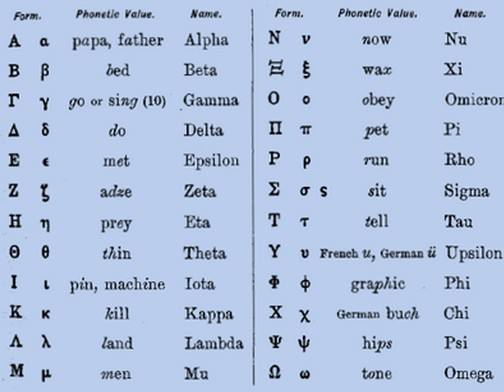
\includegraphics[width=0.9\textwidth]{img/test.jpg} \caption{图片的一个简单应用场景}
% \end{figure}

% \begin{figure}
% \centering
% \subfigure[the first subfigure]{
% 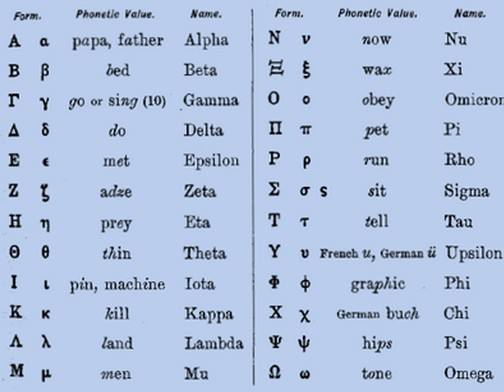
\includegraphics[width=0.4\textwidth]{img/test.jpg} 
% }
% \subfigure[the second subfigure]{
% 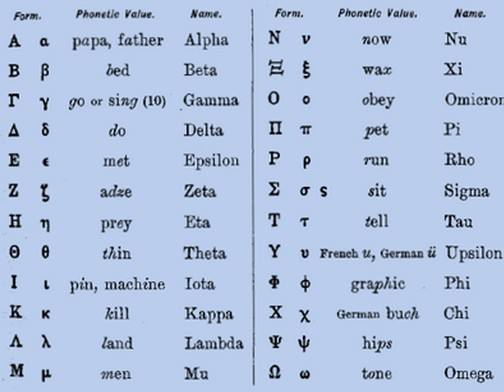
\includegraphics[width=0.4\textwidth]{img/test.jpg} 
% }
% \caption{子图应用场景}
% \end{figure}

% \section{引用论文}
% 使得论文符合要求\cite{ananthanarayanan2011scarlett}\cite{parquet}\cite{p802_3ba}。
%# -*- coding: utf-8-unix -*-
%%==================================================
%% motivation.tex for seuthesis Bachelor Thesis
%%==================================================

\chapter{研究动机}
\label{chp:motivation}


\par 过往的很多工作研究了文件的访问热度(skewed file popularities)差别很大的情况下集群缓存系统的负载均衡,在这些工作中,文件复制是被广泛应用的方法。例如,HDFS默认把一份文件复制为3份;当缓存服务器上发生缓存缺失(cache miss),Alluxio弹性增加热门文件在内存中的副本数。

\par 然而文件复制会带来较高的内存开销,最终损害缓存带来的好处。在数据分析的工作中,批处理任务分析结构化数据的情况比较多,结构化数据相比一般意义上的文件具有更多的上下文信息,其中列式存储的文件格式,比如Parquet\cite{parquet},得到越来越多的应用,因为在数据分析的大部分任务中,通常需要按列进行读取,而不是按行读取,并且列式存储把相同类型的数据归在一起,压缩比可以很高。那么问题来了,针对采用列式存储的结构化数据,我们是否能够根据其特有的性质,保证负载均衡的效果的同时,降低文件复制的开销呢?以往的研究工作表明,对一小部分热门文件(被高频访问的文件)访问占据了集群总访问量的大部分,我们猜想,那么对于结构化数据来说,例如具体一张数据表,列与列之间是否存在热门程度的差异呢?如果猜想成立,直观上来说,对于一张表,我们可以只复制最热门的几列,就能达到接近复制全表的负载均衡效果,同时能够降低缓存开销。

\par 如果按照上文所述,仅复制最热门的若干列,缓存在不同的机器上,那么在执行分布式SQL任务的时候,极有可能发生表内部的数据shuffle,我们需要探究shuffle对任务执行时间的影响。直观上来说,数据shuffle带来网络通信上的开销,会降低任务执行的效率,那么在考虑被复制的列在集群里的放置策略时,我们也需要考虑列与列之间被共同访问的概率,如果两列有很大可能性会被一起访问,那么可以考虑将它们“捆绑”(bundle)在一起放置。

\par 在本章~\ref{sec:col-access}节中,我们通过对标准基准数据集TPC系列的分析,来证明数据表中列与列之间,被访问频率存在差异,并且当考虑两两之间被共同访问的概率,两列各自的被访问频率越高,它们被共同访问的频率也越高。在~\ref{sec:data-shuffle}节中,我们通过实验证明数据shuffle会对SQL任务的执行会显著降低任务的执行效率。

\section{列的访问规律}
\label{sec:col-access}

\par 首先我们研究了具有代表性的基准标准测试程序TPC系列中的TPC-H,TPC-DS,TPC-xBB的各个数据表中的列的访问规律。

\subsection{实验设置}

\par 我们通过2.4.0版本的Spark SQL执行三种标准测试程序提供的查询任务。对于每一种,我们生成1 GB\footnote{这个实验与数据量无关,因为数据表的个数和每个表的访问规律不回随着表的规模而改变}的数据,数据存储为Parquet格式,然后将查询任务依次提交。三种标准测试程序各自包含的数据表的数量和查询任务的数量总结在表格~\ref{tab:setup}中。当执行查询任务的时候,我们记录对列的访问数据,以此来分析列级别的数据访问的性质。我们从结果中观察到以下两个现象。

\begin{figure}[t]
	\centering
	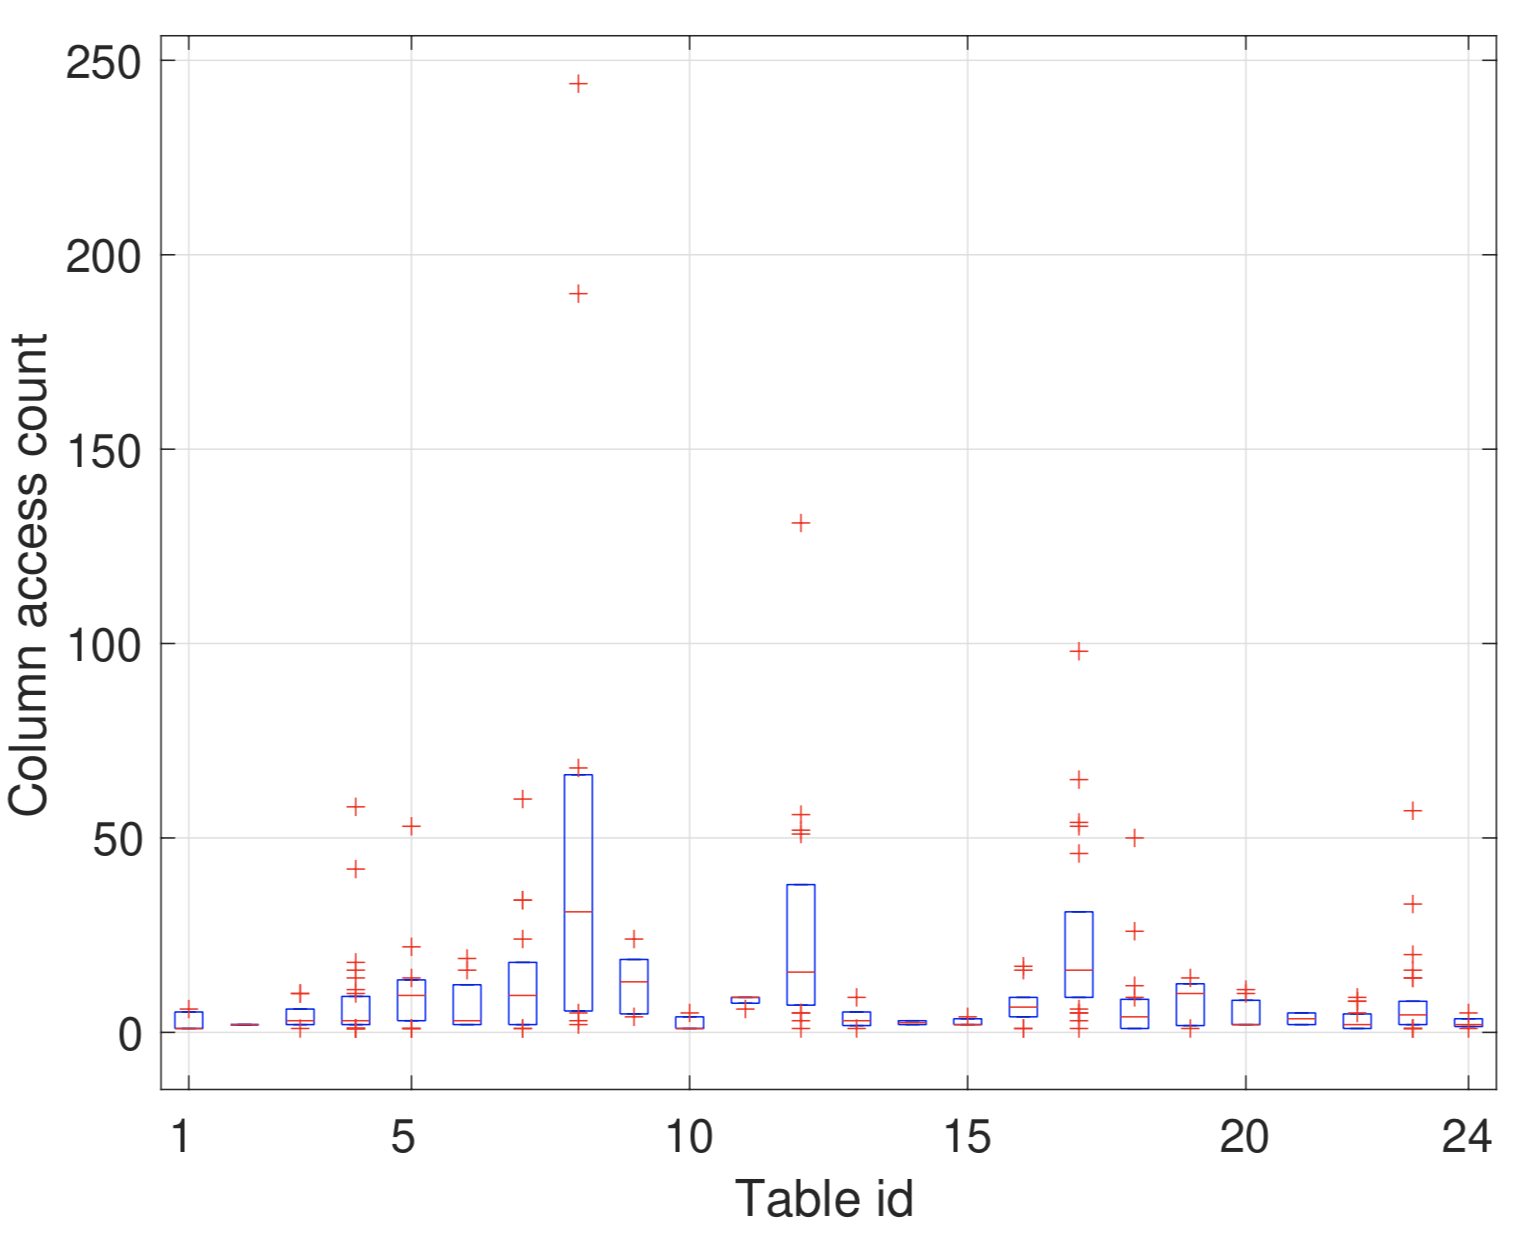
\includegraphics[width=0.5\textwidth]{img/motivation/column-pop}
	\caption{TPC-DS标准测试程序中所有数据表的列访问计数的分布。箱形图展示了每张数据表里$25$\textsuperscript{th}分位,中位数和$75$\textsuperscript{th}分位的列访问次数计数。红色标记表示离群值。}
	\label{fig:tpc-ds-column-pop}
	%\vspace{-.1in}
\end{figure}

\subsection{文件内列访问频率偏差}

\par 在上述三种标准测试程序中,我们观察到,每张数据表内,列的访问频率存在显著差异,即每张表里只有一小部分列被经常访问,而其他的列访问频次比较低。为证明这点,我们对三种标准测试程序中各数据表的列的访问进行了计数。图~\ref{fig:tpc-ds-column-pop}展示了TPC-DS标准测试程序中每张表中列访问计数的分布,箱形图展示了每张数据表里$25$\textsuperscript{th}分位,中位数和$75$\textsuperscript{th}分位的列访问次数计数。每个红色标记表示异常值,特别地,在箱形图上方的红色标记代表该表中访问频率特别高的列。从图上可以看出,对于TPC-DS的多数表,箱形图上方的红色标记远远高于箱形图顶部,这些“热门”的列被访问的次数远远超过均值,这说明文件内列访问频率存在显著偏差。此外,对于各个表而言,表越“热门”(它的列整体上访问频率高),列之间访问频率的差异越大。

\begin{table}[tbp]
    \centering
    \caption{三种标准测试程序的数据}
      \begin{tabularx}{.7\textwidth}{|l|X|X|X|r|}
      \hline
      \textbf{标准测试程序} & \textbf{表的数量} & \textbf{查询任务的数量}  \bigstrut\\ %
      \hline
      TPC-DS & 24  & 99 \bigstrut\\ %
      \hline
      TPC-H & 8  & 22 \bigstrut\\ %
      \hline
      TPC-xBB & 19  & 30 \bigstrut\\ %
      \hline
      \end{tabularx}%
      %\end{tabularx}
    \label{tab:setup}
\end{table}


\par 相似的性质也能在另外两种标准测试程序中看到,图~\ref{fig:count-cdf}展示了三种基准测试程序中所有列的访问计数的总体分布。我们发现,多数的列是“冷门的”,有很多列的访问次数是1,甚至是0,这在TPC-DS(图~\ref{fig:ds-count-cdf})和TPC-xBB(图~\ref{fig:bb-count-cdf})中表现比较明显,而一小部分列有非常高的访问计数。例如,在TPC-DS中,最“热门”的列被访问了多达$89$次。


\begin{figure}[]
    \centering
    \begin{subfigure}[t]{0.5\textwidth}
        \centering
        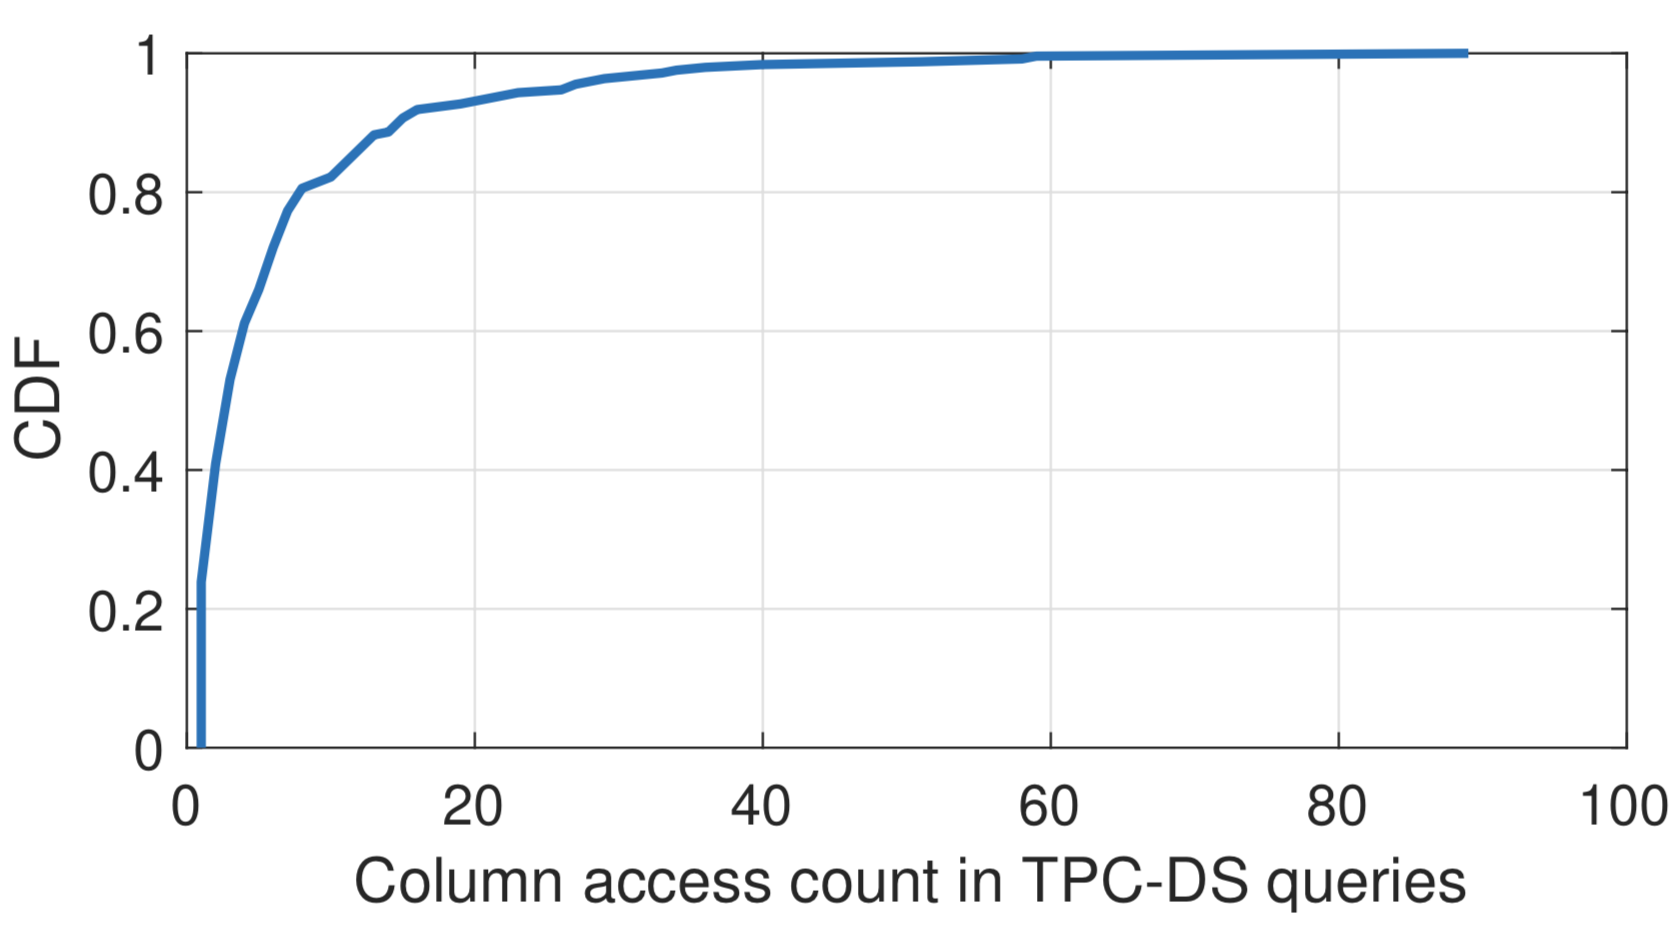
\includegraphics[width=1\textwidth]{img/motivation/ds-count-cdf}
        \caption{TDC-DS.}
        \label{fig:ds-count-cdf}
    \end{subfigure}%

    \begin{subfigure}[t]{0.5\textwidth}
        \centering
        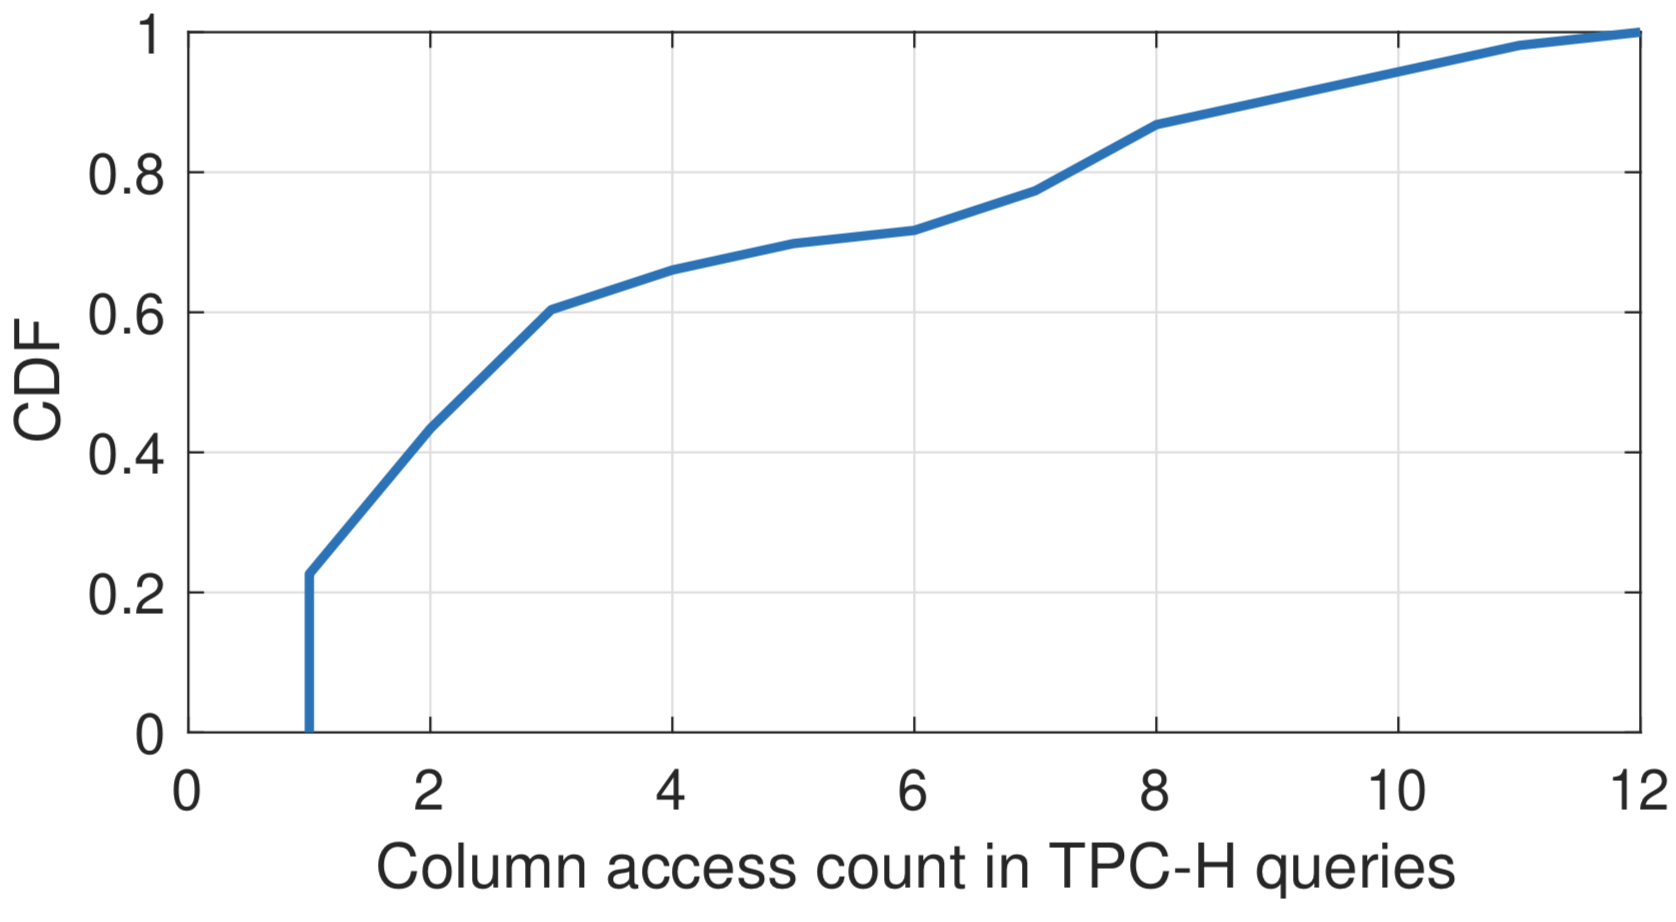
\includegraphics[width=1\textwidth]{img/motivation/h-count-cdf}
        \caption{TDC-H.}
        \label{fig:h-count-cdf}
    \end{subfigure}%

    \begin{subfigure}[t]{0.5\textwidth}
        \centering
        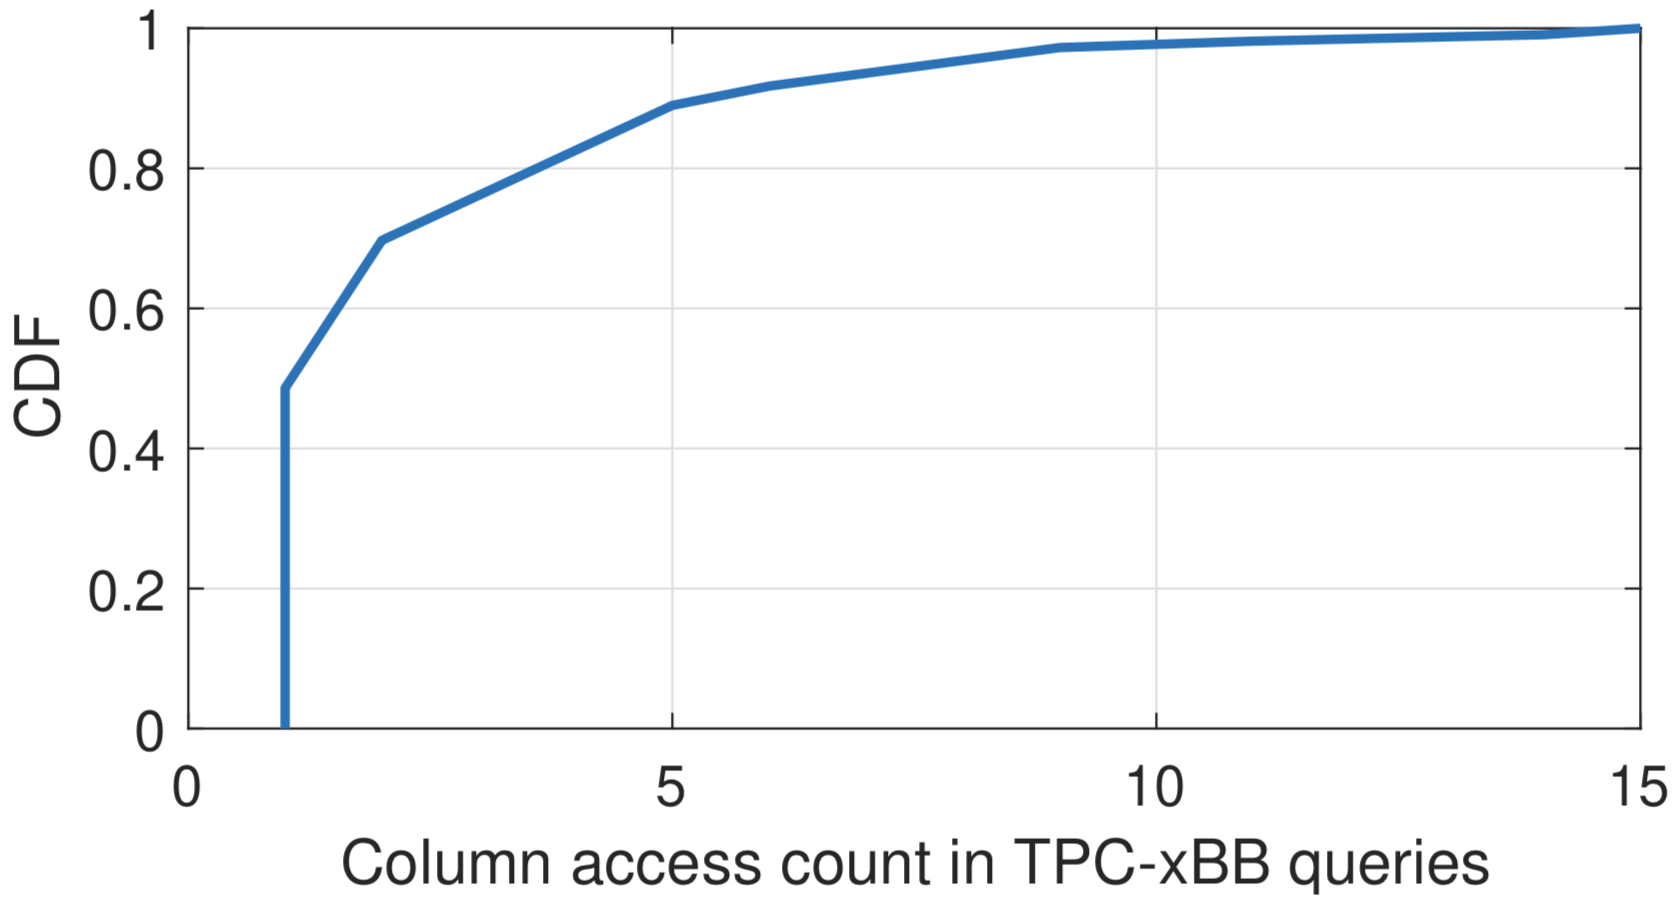
\includegraphics[width=1\textwidth]{img/motivation/xbb-count-cdf}
        \caption{TDC-xBB.}
        \label{fig:bb-count-cdf}
    \end{subfigure}%
    \caption{三种标准测试程序中列访问计数的CDF。}
    \label{fig:count-cdf}
    %\vspace{-.1in}
\end{figure}


\subsection{热门的列被共同访问的规律}
我们观察到的另一个现象是在SQL查询中,“热门”的列有很大概率会被共同访问。为了展示这一点,我们按照列的“热门程度”(访问频次)对列进行排序,绘制访问热图。我们从三个标准测试程序中各选出了一张具有代表性的表,并把结果展示在图~\ref{fig:heatmap}中。在热图里,格 $(i,i)$ (也就是对角线上的格子)代表第$i^{th}$热门的列的访问计数,格子$(i,j)$表示第$i^{th}$热门和第$j^{th}$热门的列在同一个查询任务中被共同访问的概率。从图中可以看出,每张表中越是热门的列,被共同访问的概率越高。

\begin{figure}[]
    \centering
    \begin{subfigure}[t]{0.5\textwidth}
        \centering
        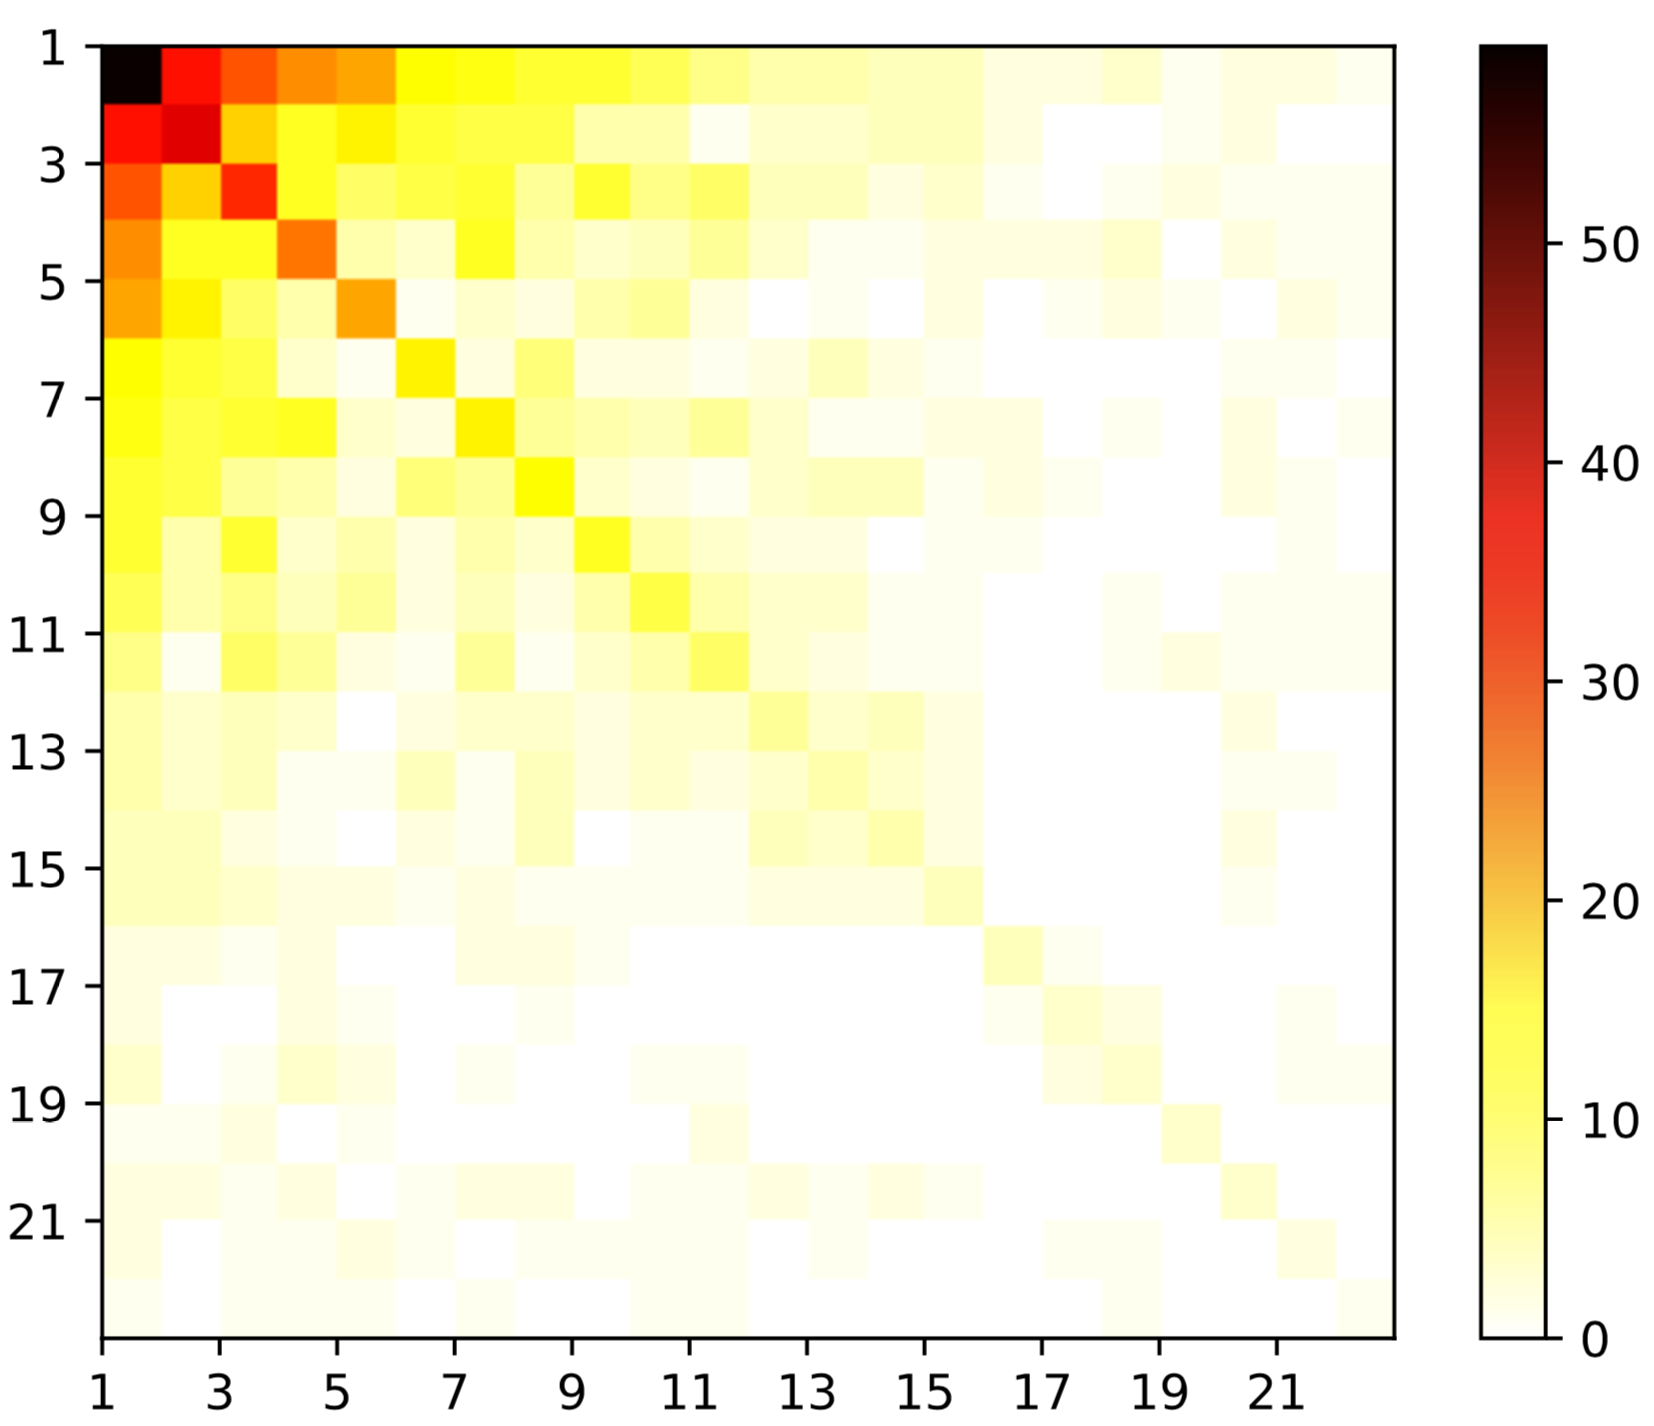
\includegraphics[width=1\textwidth]{img/motivation/tpc-ds-store_sales}
        \caption{TDC-DS中的 $store\_sales$ 表。}
        \label{fig:ds_count_cdf}
    \end{subfigure}%

    \begin{subfigure}[t]{0.5\textwidth}
        \centering
        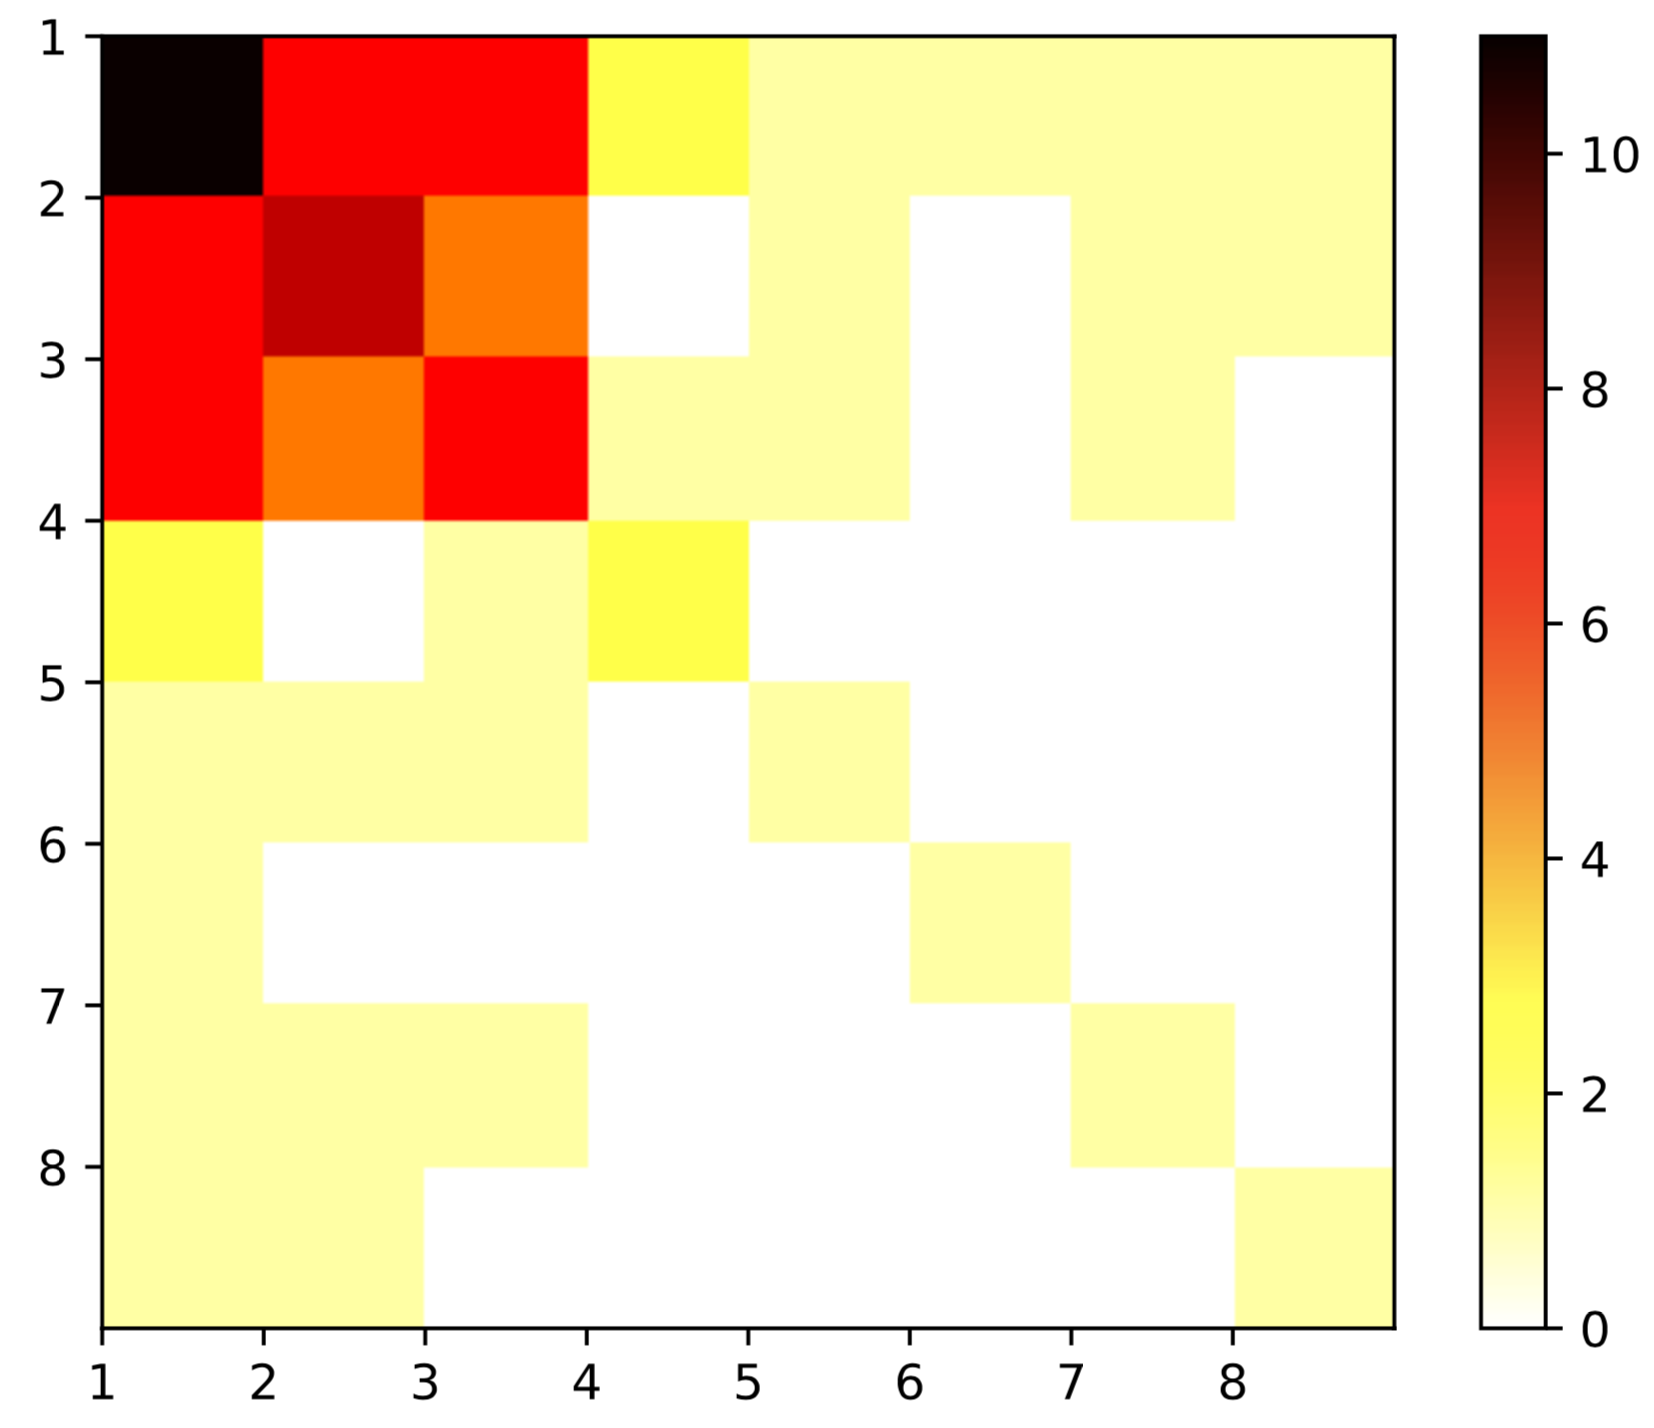
\includegraphics[width=1\textwidth]{img/motivation/tpc-h-orders}
        \caption{TDC-H中的 $orders$ 表。}
        \label{fig:h_count_cdf}
    \end{subfigure}%

    \begin{subfigure}[t]{0.5\textwidth}
        \centering
        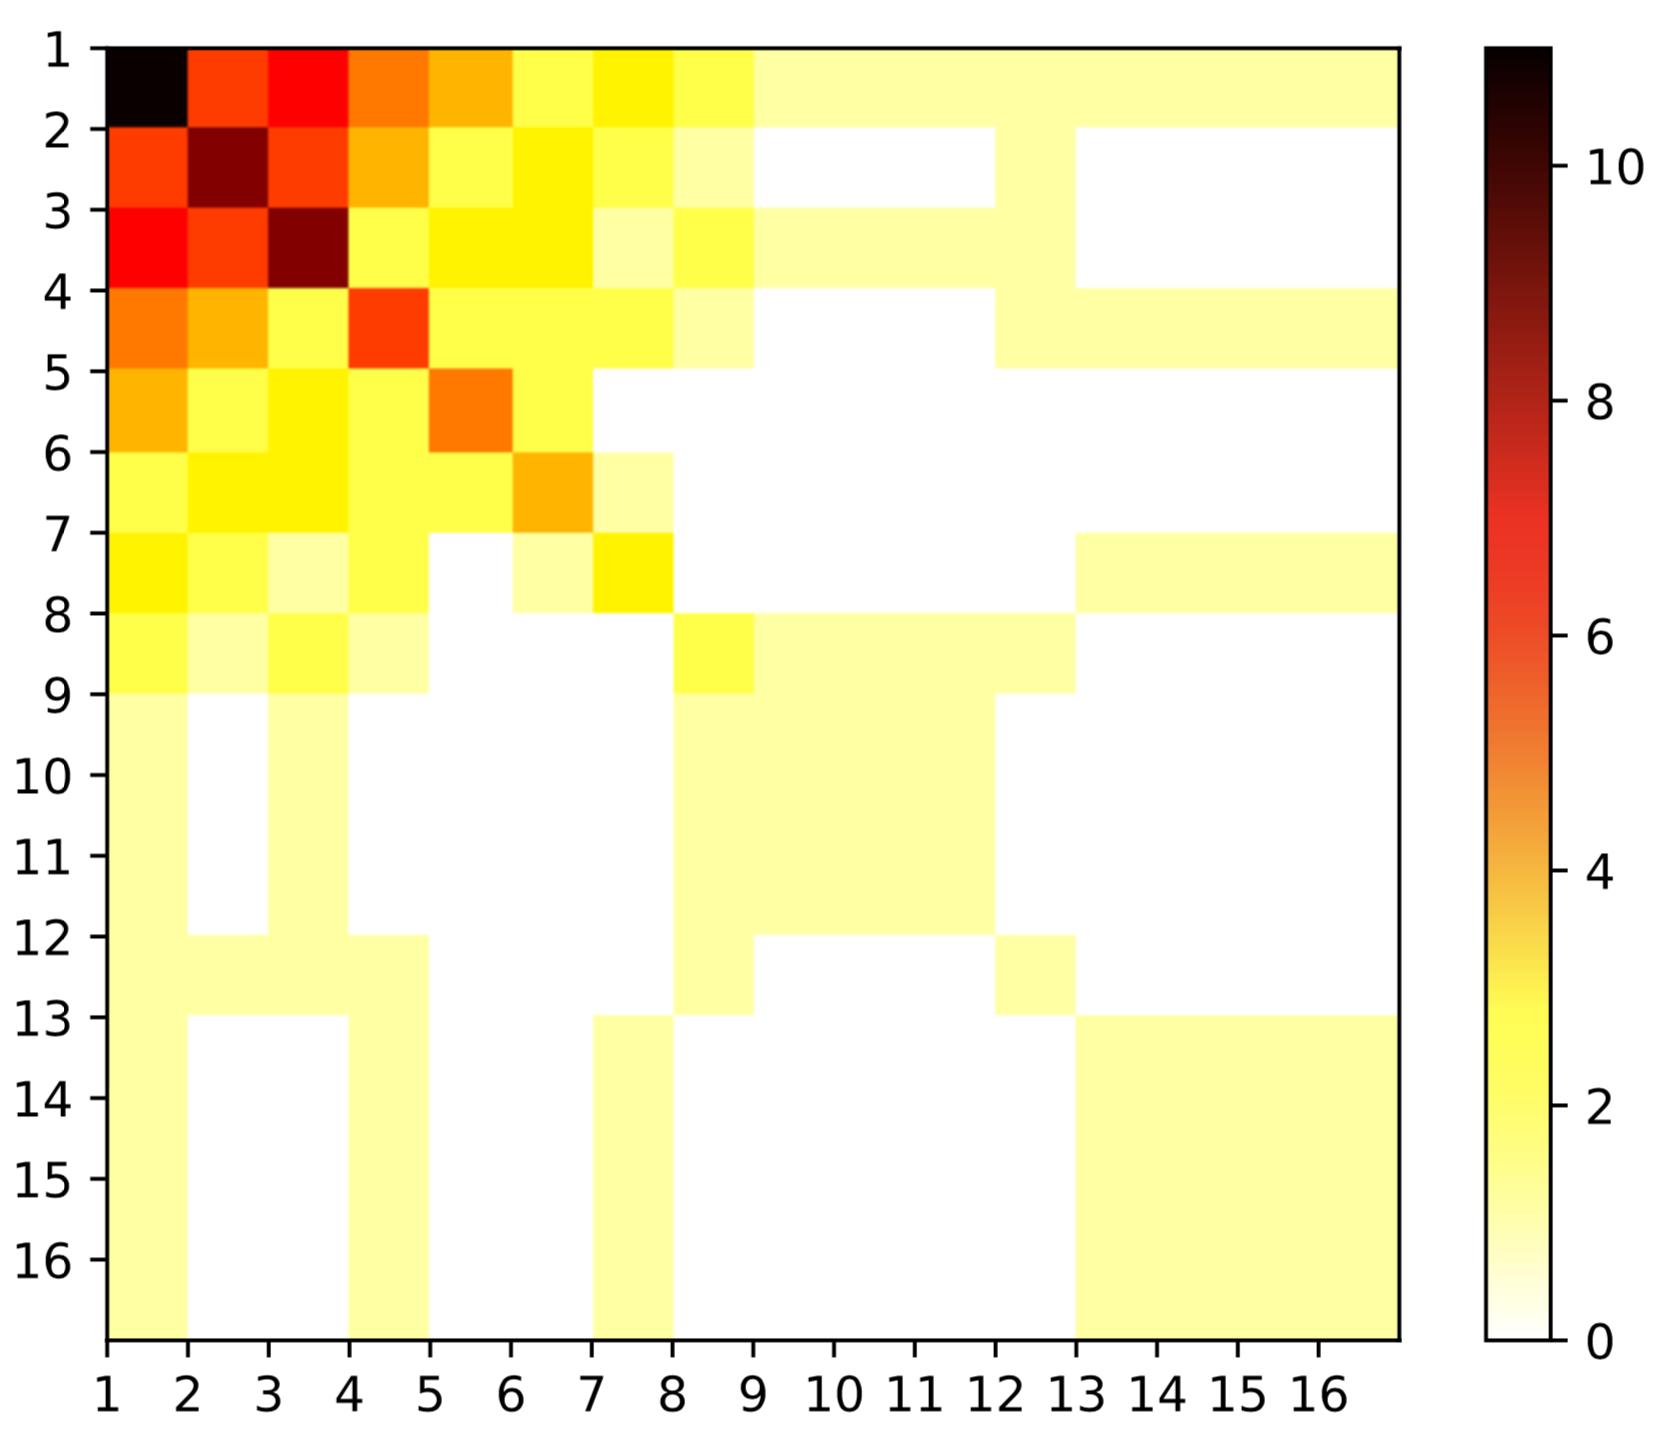
\includegraphics[width=1\textwidth]{img/motivation/tpc-bb-store_sales}
        \caption{TDC-xBB中的 $store\_sales$ 表。}
        \label{fig:bb_count_cdf}
    \end{subfigure}%
    \caption{三种标准测试程序中具有代表性的数据表的访问热图。}
    \label{fig:heatmap}
    %\vspace{-.1in}
\end{figure}

\section{列之间的数据shuffle}
\label{sec:data-shuffle}

\par 从~\ref{sec:col-access}节中观察到的现象我们获悉,每张数据表中一小部分的列非常热门,访问频率很高。如果我们复制这一小部分热门的列,并将它们缓存在不同的机器上,那么当SQL查询任务在分布式环境中执行时,这些热门的列很容易引起集群节点之间的数据shuffle。我们推测,这种shuffe给任务执行时间带来的影响是不可忽视的,为了展示列这一级别的网络开销,我们做了一个实验,测量一个小集群中列的热门程度与数据shuffle的关系。

\subsection{实验设置}
\label{subsec:data-shuffle-setup}

\par 我们部署了一个含有1个master和2个worker的小集群,所用的实例是c5.4xlarge,每一个有32 GB内存和16个CPU核,通过iperf3测试,小集群的网络带宽是10 Gbps。我们在集群上部署了Alluxio以及Spark,运行TPC-H标准测试程序。在实验中,只有一台worker缓存有6 GB的Parquet格式的数据,因此集群里每次执行查询任务都会引发从有数据的机器到没有数据的机器的数据shuffle。我们关闭了Spark和Alluxio的数据被动缓存功能,一个一个按顺序执行标准测试程序里的查询任务,保证每一次执行都会有数据shuffle。我们会记录每一列的总shuffle量。

\begin{figure}[htbp]
	\centering
	\begin{subfigure}[t]{0.5\textwidth}
		\centering
		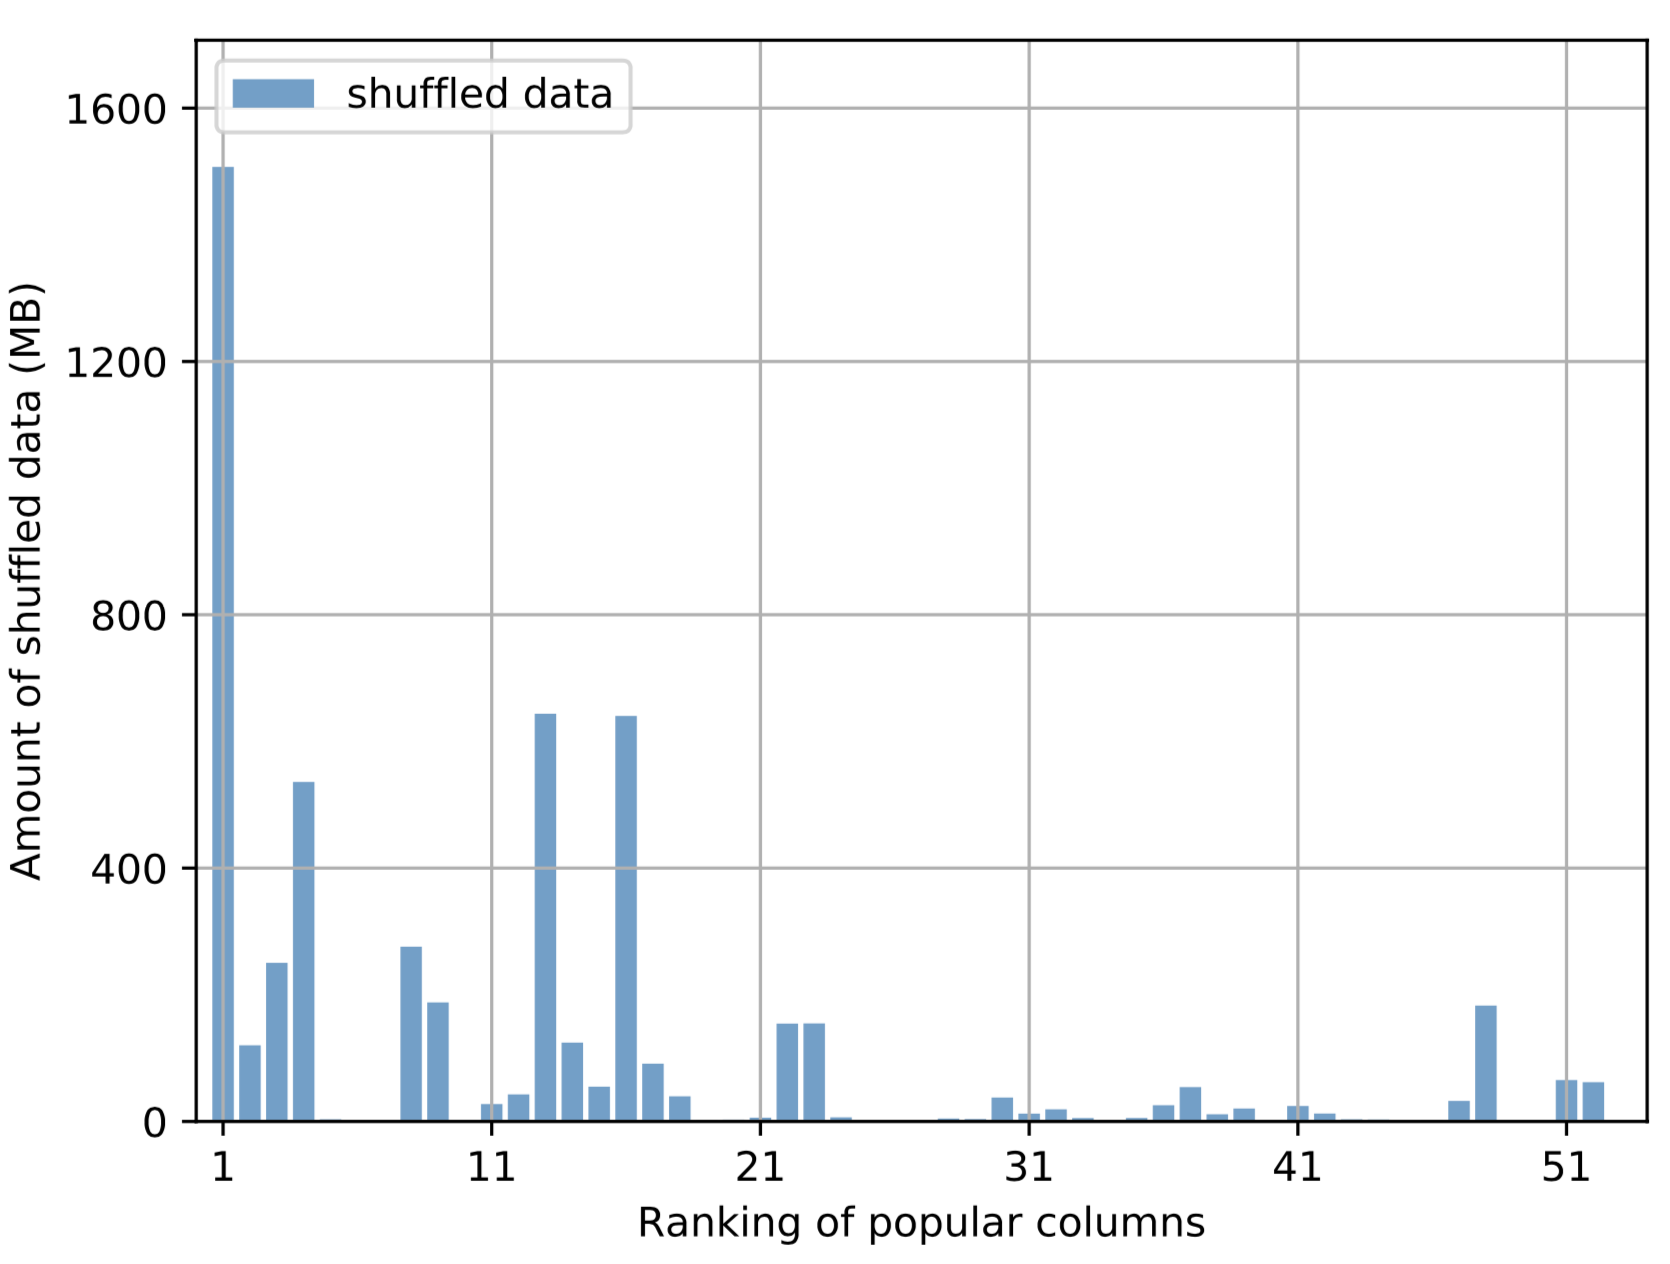
\includegraphics[width=1\textwidth]{img/motivation/pop-shf-a}
		\caption{每一列的总shuffle数据量。}
		\label{fig:pop-shf-a}
	\end{subfigure}%
	\begin{subfigure}[t]{0.5\textwidth}
		\centering
		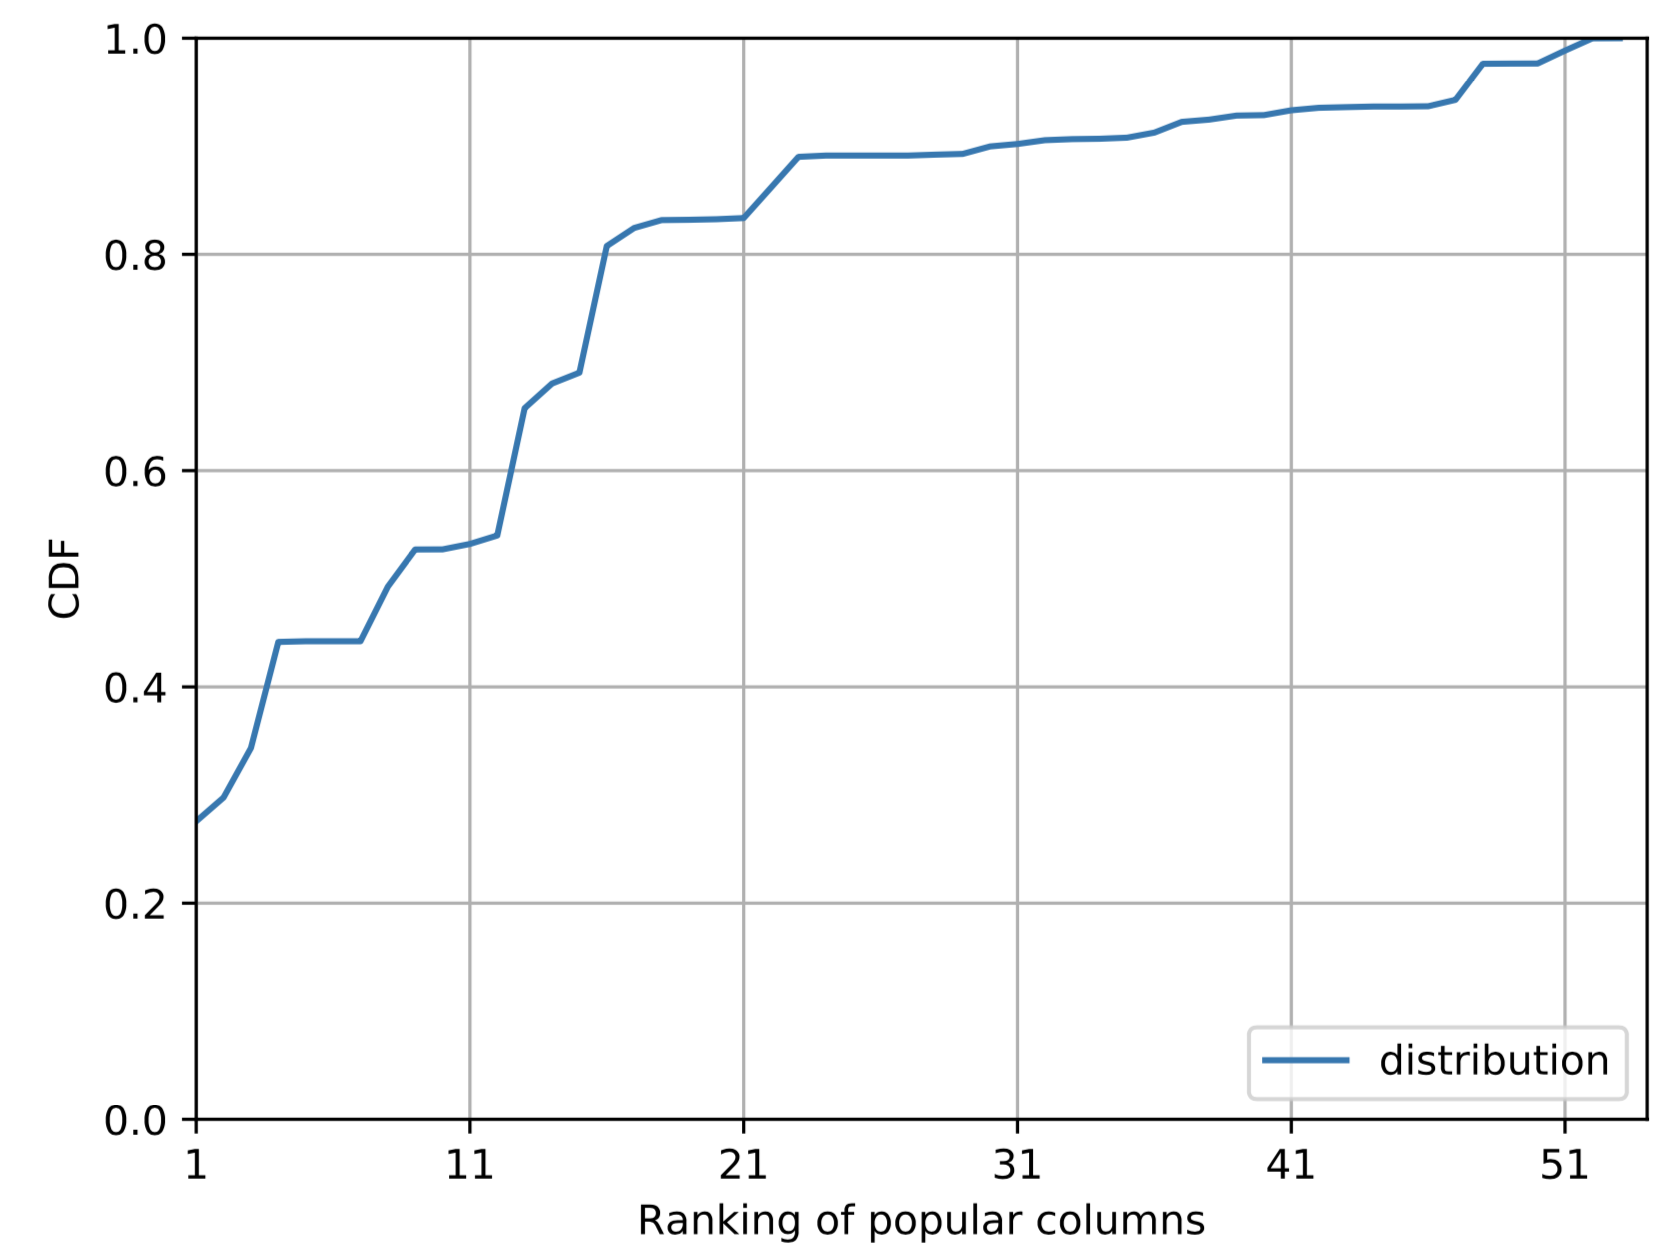
\includegraphics[width=1\textwidth]{img/motivation/pop-shf-b}
		\caption{列级别shuffle数据的CDF。}
		\label{fig:pop-shf-b}
	\end{subfigure}%
	
	\caption{TPC-H标准测试程序的列级别数据shuffle。}
	\label{fig:pop-shf}
	%\vspace{-.1in}
\end{figure}



\subsection{每一列的数据shuffle}

\par 图~\ref{fig:pop-shf}展示了上述实验的结果,其中图~\ref{fig:pop-shf-a}展示了列这一级别的数据shuffle量,TPC-H标准格式程序中的53列(所有表中的)按照它们的热门程度排序。因为热门的列被频繁访问,并且我们发现通常来说热门的列比冷门的列的体积更大,所以热门的列相比冷门的列引起更多的数据shuffle。根据图~\ref{fig:pop-shf-b}展示的分布,总体来说,查询任务产生的数据shuffle主要来自热门的列,比如接近90\%的数据shuffle量是由30\%最热门的列贡献的。

\section{数据shuffle的影响}
\label{sec:shuffle-impact}

\par ~\ref{sec:data-shuffle}节实验证明了热门的列很容易引起数据shuffle,本节中我们会用实验证明数据shuffle会降低执行查询任务的性能。

\subsection{实验设置}
\label{subsec:shuffle-impact-setup}

\par 这个实验所用的集群与~\ref{subsec:data-shuffle-setup}小节中描述的集群一致。我们设置了对照实验,其中实验组的设置与~\ref{subsec:data-shuffle-setup}小节一致,只把数据缓存在一台worker上,这一组会产生数据shuffle;另外一组中,我们将相同的数据在两台worker上均进行缓存,保证不会产生数据shuffle。我们对比两组中查询任务的执行时间,以此测量shuffle的开销。

\subsection{度量指标}
\label{subsec:shuffle-impact-metrics}

\par 我们使用任务的平均执行延迟\emph{slowdown}作为衡量指标:
\begin{equation}
    \text{Slowdown} = \frac{L_S - L_N}{L_N},
    %\text{Slowdown} = \frac{L_S - L_N}{L_N} \times 100\%,
\end{equation}

\par 其中$L_S$ 和 $L_N$ 分别是由shuffle和没有shuffle的实验中查询任务的执行时间。\emph{slowdown}的值越大表明其降低查询任务执行的性能的影响越显著。

\subsection{不同网络带宽下的shuffle开销}

\par 按照~\ref{subsec:shuffle-impact-setup}小节的设定,我们依次执行了TPC-H标准测试程序提供的查询任务并计算了每个查询任务的\emph{slowdown}(~\ref{subsec:shuffle-impact-metrics})。图~\ref{fig:cdf16-all}展示了网络带宽被限制为1 Gbps,3 Gbps和10 Gbps的情况下,\emph{salowdown}的分布。从图中可以看出,对于分布式环境下执行的SQL查询任务,网络是瓶颈,所以数据shuffle大大影响了任务执行的性能。例如,即便是在10 Gbps的带宽下,40\%的查询任务的延迟由于数据shuffle会上升10\%。此外,当网络带宽变得越小,shuffle带来的通信开销会更加明显,任务的性能的下降也会更加显著。



\begin{figure}[]
	\centering
	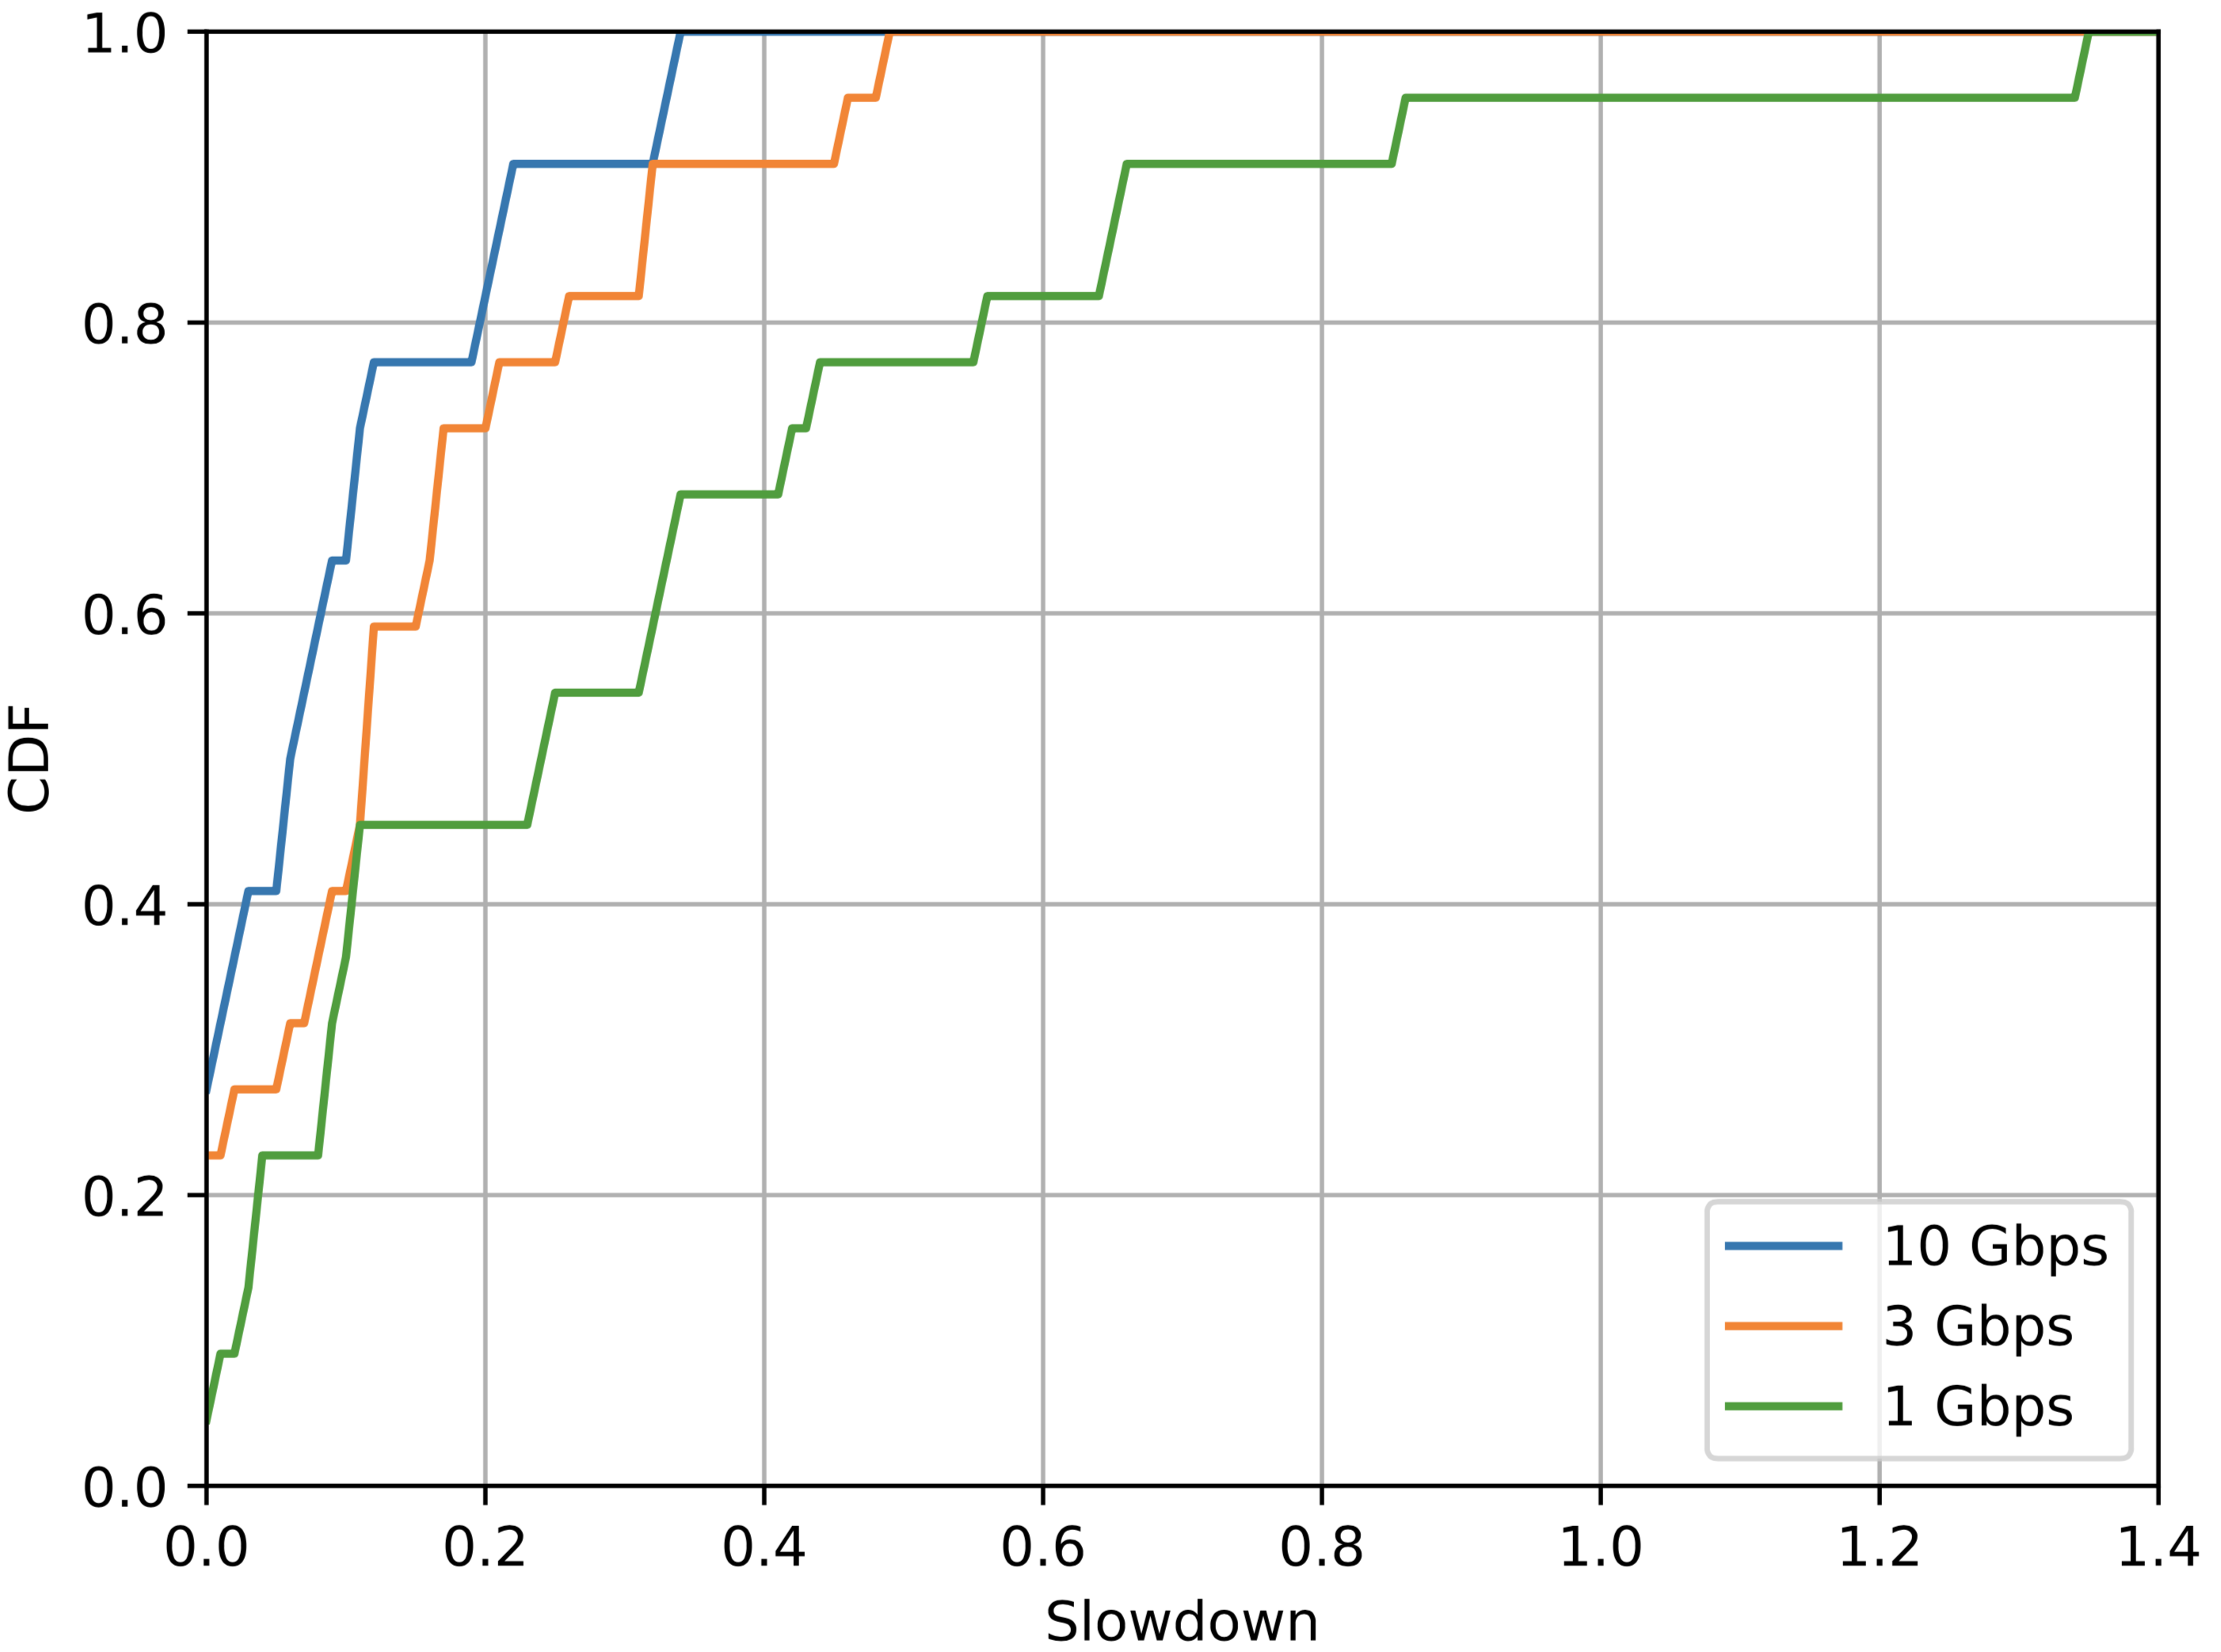
\includegraphics[width=0.5\textwidth]{img/motivation/cdf16-all}
	
	\caption{slowdown在不同网络带宽下的分布。}
	\label{fig:cdf16-all}
	%\vspace{-.1in}
\end{figure}

\section{总结}

\par 我们从本章第~\ref{sec:col-access}节得知,一张数据表中不同列之间热门程度(访问频率)存在明显的差异,且当考虑两两之间被共同访问的概率时,两列的热门程度越高,二者被共同访问的频率越高。在一张表中,热门的列是少数,其余多数是冷门的,不经常被访问。我们这些规律可以推断,相比对整张数据表进行复制,理论上复制数据表里相对热门的若干列能够达到接近复制整表的负载均衡的效果。因为冷门的列本身访问次数不多,在较长的一段周期内,热门的列的访问负载由其副本承担,而冷门的没有被复制的列的访问负载由原表承担,直观来说,这能够起到不错的负载均衡效果。与此同时,复制更少的列,降低缓存开销。提高缓存效率。

\par 将热门的列分别复制,如果随机放置在缓存服务器上,那么一个查询任务很容易引起表内部的数据shuffle,因为各个列的副本很有可能不在同一台服务器上。第~\ref{sec:data-shuffle}节显示,通常来说,热门的列引起的数据shuffle的量更大,第~\ref{sec:shuffle-impact}节证明,表内部的数据shuffle对于查询任务的执行时间的影响是不可小觑的。

\par 以上总结告诉我们,设计方案时我们需要考虑:第一,哪些列是热门的列,需要复制多少热门的列;第二,复制以后,这些列在集群里如何放置,这涉及到“捆绑”(bundle)放置的问题。

\end{Main} % 结束正文

\begin{Acknowledgement}{}
    这次的毕业论文设计总结是在我的指导老师xxx老师亲切关怀和悉心指导下完成的。从毕业设计选题到设计完成,x老师给予了我耐心指导与细心关怀,有了莫老师耐心指导与细心关怀我才不会在设计的过程中迷失方向,失去前进动力。x老师有严肃的科学态度,严谨的治学精神和精益求精的工作作风,这些都是我所需要学习的,感谢x老师给予了我这样一个学习机会,谢谢!
    
      感谢与我并肩作战的舍友与同学们,感谢关心我支持我的朋友们,感谢学校领导、老师们,感谢你们给予我的帮助与关怀;感谢肇庆学院,特别感谢计算机科学与软件学院四年来为我提供的良好学习环境,谢谢!
\end{Acknowledgement}

% 参考文献
\bibliography{seuthesis}

\begin{Appendix}
\chapter{1}
hello1
\chapter{2}
hello2
\end{Appendix}

\newpage
\printindex % 索引

%\begin{thebibliography}{99}


%\bibliographystyle{ieee}
%\bibliography{seuthesis}


\end{document}
